\documentclass[12pt]{report}
\usepackage[T1]{fontenc}
\usepackage[utf8]{inputenc}
\usepackage[spanish,es-tabla]{babel}
\usepackage{graphicx}
\usepackage[table]{xcolor}
\usepackage{fourier}
\usepackage{multirow}
\usepackage{stackengine,amsmath,amsfonts,amssymb,braket}
\usepackage{gensymb,wrapfig,enumitem}
\usepackage{pgfgantt,rotating,array}
\usepackage{booktabs,longtable}
\usepackage{placeins} % \FloatBarrier: evita que tablas/figuras crucen secciones
% Marcador de cita pendiente: resalta en el PDF y es greppable en el fuente.
% Cada \needcite corresponde a una fuente que el autor debe localizar y agregar
% a bibliografia.bib, reemplazando el marcador por el \cite correspondiente.
\newcommand{\needcite}[1]{\textbf{\textcolor{red}{[CITA: #1]}}}
\definecolor{ucmblue}{RGB}{0,85,150}
\definecolor{obj1}{HTML}{1F77B4}
\definecolor{obj2}{HTML}{FF7F0E}
\definecolor{obj3}{HTML}{2CA02C}
\definecolor{general}{HTML}{7F7F7F}
\usepackage[pdfborder={0 0 0}]{hyperref}
\usepackage{xurl} % permite partir URLs largas en la bibliografia (evita desbordes)
\usepackage{fancyhdr}
\pagestyle{fancy}
\usepackage[letterpaper,top=1.36in,left=1.18in,headheight=2in]{geometry}
% --- ABOUT -----
% Formato proyecto de título para ICI-UCM
% ver.0.1 -by Javier Rojas (jerojas@ucm.cl)

\fancyhf{}
%\fancyhead[L]{\includegraphics[height=0.8in]{logos_UCM_Fac_Cs_de_la_Ingenieria.png}}
\renewcommand{\headrulewidth}{0pt}
\renewcommand\thetable{\thesection.\arabic{table}}
\renewcommand\thefigure{\thesection.\arabic{figure}}  
\counterwithout*{section}{chapter}

% --- Rellenar datos del encabezado
\title{Análisis comparativo de un enfoque multi-sitio frente a modelos locales para la proyección a corto plazo de generación fotovoltaica bajo escasez de datos} % Título del trabajo
\date{Junio 2026} % Fecha del trabajo
\newcommand{\estudiante}{César David Aular Muñoz} % Nombre del estudiante
\newcommand{\guia}{Dr. Sergio Hernández Álvarez} % Nombre del profesor Guia
\newcommand{\revis}{Dra. Xaviera Lopez Cortés}
\newcommand{\reviss}{Dr. Juan Luis López Díaz}
%\newcommand{\revisss}{PROFESOR COMISIÓN} %Si requirere agregar más, descomente esta linea
\newcommand{\carrera}{INGENIERÍA CIVIL INFORMÁTICA} % Carrera
%\includeonly{cap1,cap2} % En caso de querer compilar solo ciertos capitulos

%--- Sección de formato (NO MODIFICAR)

\begin{document}
\pagenumbering{Roman}
{
  \makeatletter
  \newcommand{\motivo}{Proyecto de título para optar al Título de Ingeniero Civil Informático}
  \ \vspace{-1cm}\\
  {\centering
\includegraphics[width=4cm]{logo_ucm}\\}
  \vspace{0.5cm}
  \begin{center}
    {\large
    \textbf{UNIVERSIDAD CATÓLICA DEL MAULE}\\
    FACULTAD DE CIENCIAS DE LA INGENIERÍA\\
    ESCUELA \carrera\\\vspace{1.5cm}
    \textbf{\LARGE\@title}\\\vspace{3cm}
    \estudiante\\
    \guia\\\vspace{\fill}
    \motivo\\\vspace{1cm}
    \textbf{TALCA, \@date}}
  \end{center}
  \newpage
  {\ \vspace{-2.5cm}\\
    \begin{center}
      
\includegraphics[width=4cm]{logo_ucm}\\
      {%
        \vspace{0.5cm}\textbf{UNIVERSIDAD CATÓLICA DEL MAULE}\\\vspace{10pt}
        FACULTAD DE CIENCIAS DE LA INGENIERÍA\\
        ESCUELA INGENIERÍA CIVIL INFORMÁTICA\\\vspace{0.7cm}}
      \motivo\\\vspace{0.5cm}
      {\bf
        \@title\\\vspace{7pt}
        \estudiante
      }
    \end{center}\vspace{1.0cm}
  }
  {%
    \noindent\begin{tabular}{p{0.7\textwidth}c}
      \textbf{COMISIÓN EXAMINADORA}&
                                     \begin{minipage}{0.3\textwidth}
                                       \centering\textbf{FIRMA}
                                     \end{minipage}\\
      \vspace{10pt}PROFESOR GUÍA\vspace{5pt}\newline\guia &\\\cline{2-2}
      \vspace{10pt}PROFESOR COMISIÓN\vspace{5pt}\newline\revis &\\\cline{2-2}
      \vspace{10pt}PROFESOR COMISIÓN\vspace{5pt}\newline\reviss &\\\cline{2-2}
%      \vspace{10pt}PROFESOR COMISIÓN\vspace{5pt}\newline\revisss &\\\cline{2-2} % Quitar comentario en caso de agregar otro miembro a la comision
    \end{tabular}\vspace{\fill}\\
    \begin{tabular}{p{0.7\textwidth}c}
      NOTA FINAL EXAMEN DE TÍTULO:&
                                    \begin{minipage}{0.3\textwidth}
                                      \
                                    \end{minipage}\\\cline{2-2}
    \end{tabular}
    \begin{center}
      \vspace{10pt}TALCA, \@date
    \end{center}
  }
  \makeatother
}
\newpage
\section*{AGRADECIMIENTOS}
Al mirar en retrospectiva, la nostalgia se mezcla con una profunda gratitud. Este proceso, forjado entre cumbres y valles, ha sido un viaje hermoso que me ha transformado por completo.

A mi familia, mi agradecimiento más profundo: sin ustedes simplemente no estaría aquí. Tras sobrepasar tifones y cruzar incesantes tormentas, han sido la base inquebrantable de luz que me permitió mantenerme en pie y seguir adelante.

A mis amigos, testigos de mi crecimiento y compañeros de trinchera en cada batalla, victoria y derrota. Ha sido un privilegio verlos convertirse en personas maravillosas que, estoy seguro, lograrán cosas asombrosas.

A mis compañeros, por demostrarme en la práctica que la competencia y el trabajo en equipo son fuerzas perfectamente complementarias.

A la Universidad Católica del Maule, por enseñarme que la excelencia no es un destino, sino un camino; y es la convicción inquebrantable de recorrerlo la que nos propulsa hacia cosas mejores.

A mis profesores, por brindarme la guía y las herramientas para avanzar; su rigor y conocimiento han sido los cimientos sobre los cuales he podido construir este logro. Un reconocimiento especial a mi profesor guía: ha sido un verdadero honor trabajar a su lado. Su vasta experiencia, sus agudas críticas y su excelente disposición y buena voluntad fueron el catalizador de este trabajo.

Mi gratitud también se extiende al Estado de Chile, por abrirme sus puertas y acogerme de forma plena, permitiéndome echar raíces en su cultura y su sociedad.

En un acto de justicia con este proceso, también me agradezco a mí mismo. Por la perseverancia, el sacrificio y la valentía de no rendirme ante la exigencia. Por creer en mí antes que nadie, mantener la humildad para ayudar y ser ayudado, y por la determinación de aprender de todo para caminar hacia adelante, persiguiendo incansablemente la convicción de ser mejor.

Finalmente, este documento es la culminación de una etapa, pero no el final del viaje. Es apenas el génesis de un camino nuevo, mucho más desafiante y ambicioso. Que este logro no sea un punto de llegada, sino el impulso definitivo para conquistar metas cada vez mayores.

\newpage
\section*{RESUMEN}
Elabore un resumen de no más de 300 palabras de su proyecto de título. Considere que este resumen debe contener los siguientes elementos:

\begin{itemize}
\item Contextualizar el problema, explicar la importancia del problema e indicar el problema actual a resolver.
\item Mencionar los principales materiales, métodos y/o metodologías utilizadas para resolver el problema.
\item Indicar los posibles resultados.
\item Recuerde escribir en tercera persona
\item \colorbox{yellow}{Borre el texto que no es suyo y comience a escribir.}
\end{itemize}
\newpage
\section*{ABSTRACT}
En base al resumen del Ítem anterior elabore un abstract de no más de 300 palabras en el idioma inglés.

\begin{itemize}
\item No copiar directamente de traductores online.
\item \colorbox{yellow}{Borre el texto que no es suyo y comience a escribir}
\end{itemize}

\renewcommand{\contentsname}{ÍNDICE DE CONTENIDOS}
\tableofcontents

\renewcommand{\listfigurename}{LISTA DE FIGURAS}
\renewcommand{\listtablename}{LISTA DE TABLAS}

\listoffigures

\listoftables

\chapter*{Capítulo I\\Introducción y Objetivos}
\pagenumbering{arabic}
\renewcommand{\headwidth}{\textwidth}
\renewcommand{\headrulewidth}{1pt}
\renewcommand\thesection{\arabic{section}}
\addcontentsline{toc}{chapter}{\chaptername{} I}
\fancyhead[L]{\chaptername{} \rightmark}
\fancyhead[R]{\thepage}
\fancyfoot{}

%--- FIN: Sección de formato (EVITAR MODIFICAR)
\section{Introducción y Objetivos}

\subsection{Introducción}
En las últimas décadas, la energía solar ha cobrado una gran relevancia, llegando a representar una parte sustancial de la generación de energía renovable a nivel mundial gracias a los avances en las tecnologías fotovoltaicas y a la creciente demanda energética \cite{IEA2023}. La expansión de la infraestructura de energía solar es un pilar fundamental para la electrificación, la transición energética global y el cumplimiento de los compromisos de cero emisiones netas para mitigar los efectos del cambio climático. Sin embargo, la generación fotovoltaica está sujeta a una alta variabilidad e intermitencia, ya que depende directamente de factores meteorológicos dinámicos como la Irradiancia Horizontal Global (GHI), la temperatura, la nubosidad y la velocidad del viento \cite{Antonanzas2016}. Por lo tanto, la estimación precisa de la productividad en plantas de energía renovable es un desafío crítico para la planificación, operación y optimización de los sistemas energéticos de la red \cite{cen2025}.

Tradicionalmente, los modelos predictivos de generación solar se han abordado mediante técnicas estadísticas y algoritmos clásicos que se entrenan de manera local utilizando los datos históricos específicos de cada planta. Este enfoque presenta dos limitaciones fundamentales. En primer lugar, dependen fuertemente de la disponibilidad de un volumen considerable de datos históricos locales, lo cual dificulta enormemente su aplicación en escenarios de puesta en marcha de nuevas instalaciones (el problema de \textit{cold-start} o arranque en frío). En segundo lugar, omiten el aprovechamiento de los patrones meteorológicos y operativos que son compartidos entre distintas plantas y regiones climáticas, los cuales poseen un alto valor para mejorar la capacidad predictiva y la generalización de los modelos.

Para superar estas barreras de disponibilidad de datos, la investigación reciente ha comenzado a integrar técnicas avanzadas de Deep Learning, donde arquitecturas como los Transformers (ej. Temporal Fusion Transformer, Informer \cite{Zhou2021} o PatchTST \cite{Nie2022}) han demostrado una capacidad superior para procesar secuencias largas y extraer dependencias temporales complejas a partir de datos meteorológicos multivariados \cite{Arslan2025}. Complementariamente, el uso de enfoques de \textit{Transfer Learning} (aprendizaje por transferencia) permite que un modelo pre-entrenado a partir de bases de datos a gran escala y de múltiples regiones transfiera características y patrones climáticos generales hacia instalaciones locales con escasez de datos \cite{Bak2025}.

El presente proyecto busca abordar el problema del \textit{cold-start} a través del desarrollo y validación de una arquitectura de "\textit{Cross-Site Learning}" (aprendizaje multi-sitio). Mediante el uso de un modelo Transformer de estado del arte, el proceso de entrenamiento se adaptará para aprender simultáneamente de múltiples series temporales de distintas plantas solares, integrando variables exógenas dinámicas (clima) y características estáticas (ubicación geográfica).

El desarrollo de este proyecto aporta valor empírico y metodológico en dos frentes principales. En primer lugar, proporciona una herramienta validada para la industria, permitiendo a los operadores estimar con mayor precisión la producción de nuevos parques solares desde sus etapas iniciales sin depender de recolecciones de datos locales prolongadas. En segundo lugar, aporta evidencia sólida sobre la eficacia de aplicar técnicas de \textit{Transfer Learning} y arquitecturas Transformer en series de tiempo energéticas, estableciendo un marco de evaluación riguroso frente a modelos tradicionales de Machine Learning (como XGBoost o LSTM) entrenados de manera estrictamente local.

\subsection{Problemática}
La transición hacia una matriz energética sostenible ha impulsado una expansión acelerada de proyectos fotovoltaicos. Tal como indica la Comisión Nacional de Energía, el 75\% de los 5.333 MW de nueva capacidad eléctrica actualmente en etapa de construcción en el país corresponde a parques solares \cite{cne2026}. Sin embargo, esta inyección masiva de energía choca con una barrera crítica para la toma de decisiones: la escasez de datos meteorológicos y operativos durante las etapas iniciales de un proyecto. Para generar proyecciones confiables y superar el problema del Cold-Start, los algoritmos predictivos tradicionales —entrenados de manera aislada para cada instalación— requieren de un mínimo de un año ininterrumpido de registros locales \cite{rodriguez2023energy}. Esto fomenta un profundo aislamiento del aprendizaje técnico, impidiendo que el conocimiento atmosférico generalizado (enfoque Multi-Sitio) se transfiera, lo que condena a los nuevos actores del mercado a operar con altos niveles de incertidumbre algorítmica desde su puesta en marcha.

Esta falta de predictibilidad a corto plazo desencadena severas ineficiencias operativas y un alto riesgo financiero a lo largo de la red. A nivel sistémico, el Coordinador Eléctrico Nacional (2025) reporta que las imprecisiones en los pronósticos de inyección renovable han introducido un error financiero del 4,62\% sobre la estimación de los costos operativos totales del Sistema Eléctrico Nacional. Más grave aún, la incapacidad de anticipar con exactitud la generación exacerba los cuellos de botella en la transmisión, derivando en niveles críticos de vertimiento de energía limpia (curtailment). Durante 2025, el vertimiento físico alcanzó los 6.084 GWh \cite{acera2025}, lo que se ha traducido en pérdidas de ingresos para las generadoras equivalentes a 562 millones de dólares acumulados en los últimos tres años \cite{ember2025}. Finalmente, en el ecosistema a menor escala, esta incertidumbre algorítmica expone directamente a los Pequeños Medios de Generación Distribuida (PMGD) a un riesgo de mermas financieras estimado en hasta 7.400 millones de dólares anuales ante la falta de certeza horaria en sus esquemas de inyección \cite{gpm2025}.

\begin{table}[htbp]
  \centering
  \resizebox{\textwidth}{!}{
  \begin{tabular}{|m{5cm}|m{3.5cm}|m{5.5cm}|}
    \hline
    \textbf{Variable / Métrica} & \textbf{Magnitud Estimada} & \textbf{Fuente de Referencia} \\
    \hline
    Capacidad solar en construcción & 75\% del total (MW) & Comisión Nacional de Energía (2026) \\
    \hline
    Error financiero sistémico & 4,62\% de costos operativos & Coordinador Eléctrico Nacional (2025) \\
    \hline
    Vertimiento físico anual & 6.084 GWh & ACERA (2025) \\
    \hline
    Pérdida por vertimiento (3 años)& 562 Millones USD & Ember (2025) \\
    \hline
  \end{tabular}
  }
  \caption{\label{tab:impacto_financiero} Resumen del impacto operativo y financiero por incertidumbre predictiva.}
\end{table}

\subsection{Cliente y/o Público objetivo}
El público objetivo y los principales beneficiarios de esta solución abarcan un espectro amplio dentro del ecosistema de generación de energía renovable. En primer lugar, la herramienta se orienta a operadores, administradores de parques solares a gran escala y coordinadores de redes eléctricas, quienes requieren sistemas predictivos robustos para minimizar la incertidumbre en la toma de decisiones, optimizando la planificación energética y reduciendo el riesgo financiero ante desvíos en el despacho durante las etapas iniciales de una planta.

En segundo lugar, esta propuesta integra a los actores del segmento de Pequeños Medios de Generación Distribuida (PMGD) y a los desarrolladores de sistemas de autoconsumo fotovoltaico a pequeña y mediana escala (comercial e industrial). Para este nicho, donde la instalación de sensórica avanzada o la recopilación de años de datos locales resulta económicamente inviable, un modelo multi-sitio pre-entrenado les permitirá acceder a proyecciones a corto plazo continuas y confiables desde su puesta en marcha, permitiendo rentabilizar sus operaciones y gestionar su inyección a la red sin la barrera de entrada que supone el modelado de datos aislado y tradicional.

\subsection{Objetivo General}
Analizar y comparar el desempeño de un modelo global de aprendizaje multi-sitio frente a modelos locales entrenados con datos históricos, en la estimación de la productividad de plantas de energía renovable, considerando su capacidad de generalización y su rendimiento en escenarios de escasez de datos e intermitencia.

\subsection{Hipótesis}
La implementación de un modelo globalmente entrenado con información proveniente de centros meteorológicamente variados, es capaz de usar información generalizada respecto de las variaciones en las condiciones atmosféricas para obtener un mejor resultado respecto de la producción de energía de una planta de producción desconocida, siendo más precisa que un modelo localmente entrenado solo con la información histórica del centro.

\subsubsection{Objetivos Específicos}
\begin{enumerate}
    \item Seleccionar y configurar una arquitectura Transformer preexistente que sea adecuada para el pronóstico de series de tiempo. Posteriormente, adaptar su proceso de entrenamiento con el fin de que el modelo sea capaz de procesar y aprender de manera simultánea a partir de múltiples series temporales provenientes de diferentes plantas solares, reemplazando así el tradicional enfoque de entrenamiento aislado.
    \item Evaluar la efectividad del modelo global pre-entrenado durante la puesta en marcha de una nueva planta renovable que cuente con una escasa cantidad de datos con respecto a modelos tradicionales (como XGBoost o LSTM) entrenados de manera estrictamente local.
    \item Integrar datos multimodales para dotar al modelo de la capacidad de procesar diversas fuentes de información, integrando de manera conjunta tanto variables exógenas dinámicas, que representan las condiciones meteorológicas, como características estáticas referentes a la ubicación espacial y geográfica de cada estación.
\end{enumerate}

\subsection{Alcance del Proyecto}
Con el propósito de analizar y comparar el desempeño predictivo de modelos globales frente a modelos locales, el alcance de este proyecto se focaliza en el dominio de la producción de energía solar mediante el estudio de un conjunto consolidado de instalaciones agrupadas bajo un criterio de Macrozona. Esta estrategia de agrupación responde a la necesidad de estabilizar las características climáticas compartidas y escalar el aprendizaje cruzado entre plantas. Esta configuración experimental permite integrar series de tiempo de producción y variables meteorológicas de alta fidelidad para evaluar la capacidad de generalización y la respuesta del modelo ante la escasez de datos. Técnicamente, el trabajo se concentra en la parametrización, el entrenamiento multi-sitio y la validación de arquitecturas de estado del arte (TFT, Informer, N-HiTS), empleando modelos XGBoost y LSTM como líneas base comparativas. Finalmente, para mantener el foco en la evaluación del rendimiento del modelado, se excluyen explícitamente el desarrollo de nuevas estrategias o metodologías desde cero, el despliegue en entornos de producción (MLOps), la integración con sistemas SCADA y cualquier análisis de viabilidad financiera o rentabilidad operativa sobre los activos estudiados. De manera que el proyecto se compone de la recopilación y preprocesado de datos, la configuración de la estrategia de orquestación para el testeo, el entrenamiento de los modelos base, la ejecución y posterior comparación entre el modelo globalmente entrenado y las baseline en situaciones de ``Cold-Start''. Todo circunscrito por un repositorio con los pipelines de datos, entrenamiento y posterior testeo.

\begin{figure}[htbp]
  \centering
  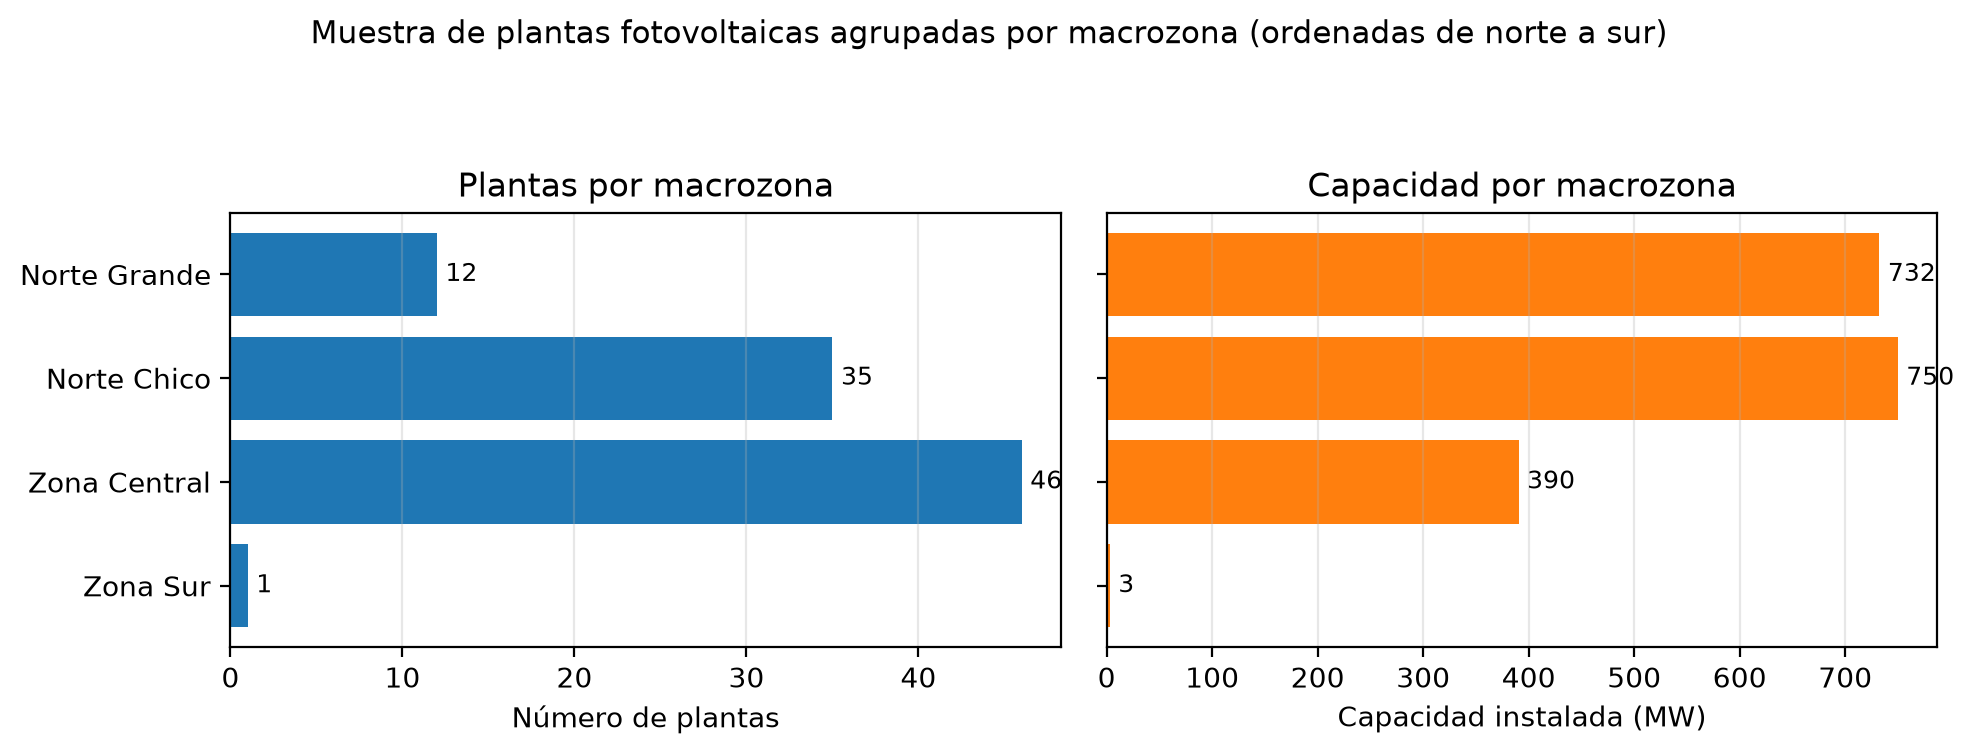
\includegraphics[width=\textwidth]{figuras/fig_mapa_muestra.png}
  \caption{\label{fig:mapa_alcance} Distribución de las plantas fotovoltaicas de la muestra por macrozona (94 instalaciones; 1.876 MW de capacidad agregada).}
\end{figure}

\subsection{Carta de Compromiso}
Dada la naturaleza de la presente investigación, el desarrollo del modelo no se encuentra aunado a la intervención o patrocinio exclusivo de una entidad privada específica para su ejecución técnica. El acceso a los activos de datos necesarios para el cumplimiento de los objetivos planteados ha sido gestionado bajo protocolos internos, lo que garantiza la viabilidad y autonomía del estudio en sus etapas de entrenamiento y validación. No obstante, se mantiene la disposición para formalizar vínculos de colaboración técnica con organismos del sector en fases posteriores, con el fin de robustecer la transferencia tecnológica de los resultados obtenidos.

\newpage

\subsection{Planificación del Trabajo (Carta Gantt)}
Para cumplir con los objetivos trazados de manera sistemática, se ha definido una carta Gantt de seis semanas de duración orientada a la ejecución técnica, evaluación del \textit{Cold-Start} y consolidación de resultados (ver Figura \ref{fig:gantt_planificacion}).

\begin{figure}[htbp]
  \centering
  \begin{ganttchart}[
      hgrid, vgrid,
      x unit=1.5cm, y unit chart=0.62cm, y unit title=0.7cm,
      title/.append style={fill=ucmblue!15},
      title label font=\small\bfseries,
      bar/.append style={rounded corners=1pt},
      bar label font=\small,
      bar height=0.6
    ]{1}{6}
    \gantttitle{Semanas de ejecución}{6} \\
    \gantttitlelist{1,...,6}{1} \\
    \ganttbar[bar/.append style={fill=obj3}]{Procesamiento de datos multimodales}{1}{2} \\
    \ganttbar[bar/.append style={fill=obj2}]{Entrenamiento algoritmos clásicos}{2}{3} \\
    \ganttbar[bar/.append style={fill=obj1}]{Parametrización arquitectura Transformer}{2}{3} \\
    \ganttbar[bar/.append style={fill=obj1}]{Entrenamiento simultáneo Cross-Site}{3}{4} \\
    \ganttbar[bar/.append style={fill=obj2}]{Simulación Cold-Start}{4}{5} \\
    \ganttbar[bar/.append style={fill=obj2}]{Benchmark comparativo y métricas}{5}{6} \\
    \ganttbar[bar/.append style={fill=general}]{Redacción y entrega final}{1}{6}
  \end{ganttchart}
  \vspace{4pt}

  {\small
    \textcolor{obj1}{$\blacksquare$}~Obj.~1: Arq.~Transformer \quad
    \textcolor{obj2}{$\blacksquare$}~Obj.~2: Eval.~Cold-Start \quad
    \textcolor{obj3}{$\blacksquare$}~Obj.~3: Datos multimodales \quad
    \textcolor{general}{$\blacksquare$}~Tareas transversales}
  \caption{\label{fig:gantt_planificacion} Planificación estructurada en 6 semanas, categorizada según los Objetivos Específicos del proyecto.}
\end{figure}

\chapter*{Capítulo II\\Marco Teórico}
\addcontentsline{toc}{chapter}{\chaptername{} II}
\section{Marco Teórico}
Este capítulo construye los fundamentos teóricos de la investigación siguiendo una progresión de lo general a lo específico: parte de la naturaleza física del recurso solar y del problema de pronóstico de series de tiempo, recorre la evolución de las técnicas predictivas —desde los modelos estadísticos clásicos hasta las arquitecturas de aprendizaje profundo basadas en atención— y culmina en el tránsito del paradigma de entrenamiento local (\textit{one-site}) al global (\textit{multi-site}), que es el eje conceptual sobre el que se articula la solución propuesta para el problema del arranque en frío.

\subsection{Generación Fotovoltaica y el Recurso Solar}
La generación de energía solar fotovoltaica corresponde al proceso de conversión directa de la radiación solar en electricidad mediante el efecto fotovoltaico. La potencia activa de salida de una planta posee una dependencia estocástica respecto a múltiples variables atmosféricas dinámicas \needcite{física del recurso solar / dependencia de la potencia FV respecto a variables meteorológicas}. La variable con mayor correlación directa es la Irradiancia Horizontal Global (GHI), definida como la cantidad total de radiación de onda corta recibida por una superficie horizontal, que integra las componentes directa y difusa \needcite{definición y componentes de la irradiancia solar (GHI, DNI, DHI)}. De forma secundaria, factores térmicos y atmosféricos como la temperatura ambiente, la humedad relativa, la velocidad del viento y, sobre todo, la nubosidad, modulan la eficiencia de conversión de los paneles \needcite{efecto de la temperatura y la nubosidad en la eficiencia fotovoltaica}. En conjunto, la intermitencia de estas variables produce fluctuaciones severas en la inyección de energía a la red, lo que convierte al pronóstico preciso de generación en un insumo crítico para la operación de los sistemas eléctricos con alta penetración renovable \cite{cen2025}.

\subsection{Series de Tiempo y el Problema de Pronóstico}
Una serie de tiempo se define como un conjunto ordenado de observaciones cuantitativas registradas en intervalos de tiempo regulares \cite{Peixeiro2022}. El pronóstico consiste en analizar estas secuencias históricas para proyectar valores futuros, tarea que se apoya en propiedades estructurales de la señal —tendencia, estacionalidad y autocorrelación— y en supuestos como la estacionariedad \cite{Peixeiro2022}. En el dominio energético, el pronóstico fotovoltaico presenta una estacionalidad múltiple y anidada (ciclo diario e interanual) y una fuerte intermitencia inducida por el clima, lo que ha motivado una progresión metodológica desde los modelos lineales clásicos hacia arquitecturas capaces de capturar dependencias no lineales de largo alcance \cite{Benidis2022}.

\subsection{Modelos Estadísticos Clásicos}
La familia de modelos estadísticos constituye el punto de partida histórico del pronóstico de series de tiempo y opera bajo un paradigma estrictamente \textbf{local}: cada modelo se ajusta a los datos históricos de una única serie, sobre la premisa de disponer de un historial largo e ininterrumpido.

El \textbf{suavizado exponencial} (\textit{exponential smoothing}) proyecta el futuro como un promedio ponderado de las observaciones pasadas, asignando pesos que decaen geométricamente hacia atrás en el tiempo; sus variantes de Holt y Holt-Winters extienden la formulación para capturar explícitamente componentes de tendencia y estacionalidad \cite{Peixeiro2022}. Por su parte, la metodología de Box-Jenkins formaliza los modelos \textbf{autorregresivos de media móvil} (ARMA) y su extensión integrada \textbf{ARIMA}, que combina términos autorregresivos, de media móvil y de diferenciación para modelar series no estacionarias \cite{Peixeiro2022}. Las variantes \textbf{SARIMA} y \textbf{SARIMAX} incorporan, respectivamente, la estacionalidad periódica y la influencia de variables exógenas (como las meteorológicas), lo que las hace teóricamente aplicables al pronóstico solar \cite{Peixeiro2022}.

La limitación fundamental de esta familia es triple: asume relaciones predominantemente lineales entre las variables, exige la satisfacción de supuestos estadísticos estrictos (estacionariedad, homocedasticidad) y, por su naturaleza local, requiere un historial extenso de la propia serie para estimar sus parámetros —condición precisamente ausente en el escenario de arranque en frío.

\subsection{Aprendizaje Automático: Ensambles de Árboles de Decisión}
La incorporación del \textit{Machine Learning} al pronóstico permitió relajar los supuestos de linealidad. Los algoritmos basados en ensambles de árboles de decisión mediante potenciación del gradiente (\textit{gradient boosting}), y en particular \textbf{XGBoost}, construyen de forma aditiva una secuencia de árboles donde cada uno corrige los errores residuales del ensamble previo, capturando interacciones no lineales entre las variables de forma eficiente y regularizada \cite{Chen2016}. En el dominio energético, estos algoritmos han demostrado un desempeño competitivo y una alta interpretabilidad al cuantificar la importancia relativa de cada variable meteorológica \cite{rodriguez2023energy}. No obstante, al ser modelos tabulares que aprenden por particionamiento del espacio de características, carecen de capacidad de extrapolación fuera del rango observado en entrenamiento, lo que degrada severamente su desempeño cuando la serie objetivo carece de historial —nuevamente, el problema del arranque en frío.

\subsection{Aprendizaje Profundo para Series Temporales}
El aprendizaje profundo (\textit{Deep Learning}) introdujo la capacidad de aprender representaciones jerárquicas directamente de los datos, superando la necesidad de ingeniería manual de características. Las redes neuronales recurrentes, y en particular la arquitectura \textbf{Long Short-Term Memory} (LSTM) \cite{Hochreiter1997}, incorporaron compuertas de memoria que permiten retener información de estados pasados y mitigar el desvanecimiento del gradiente, habilitando el modelado de dependencias temporales de corto y mediano plazo. Como alternativa a la recurrencia, las redes convolucionales temporales demostraron que arquitecturas puramente convolucionales pueden igualar o superar a las recurrentes en tareas secuenciales, con la ventaja del procesamiento paralelo \cite{Bai2018}.

Un avance conceptual relevante fue el paso del pronóstico puntual al \textbf{pronóstico probabilístico}. El modelo \textbf{DeepAR} \cite{Salinas2020} estructura una red recurrente autorregresiva que, en lugar de un único valor, estima los parámetros de una distribución de probabilidad futura, permitiendo cuantificar analíticamente la incertidumbre de la predicción —una capacidad esencial para la gestión de riesgo en la operación energética. En paralelo, las arquitecturas de expansión en bases, como \textbf{N-BEATS} \cite{Oreshkin2020}, propusieron bloques de proyección sobre bases funcionales interpretables (tendencia y estacionalidad) que alcanzaron desempeño de estado del arte sin recurrencia. Su sucesor, \textbf{N-HiTS}, refina esta idea mediante interpolación jerárquica y muestreo multi-tasa, lo que reduce drásticamente el costo computacional en horizontes largos y lo posiciona como una contraparte moderna y eficiente frente a los modelos atencionales \cite{Challu2023}. Una revisión sistemática del campo documenta esta transición y consolida al aprendizaje profundo como el paradigma dominante en el pronóstico de series de tiempo a gran escala \cite{Benidis2022}.

\subsection{El Mecanismo de Atención y las Arquitecturas Transformer}
La arquitectura \textbf{Transformer} \cite{Vaswani2017} representó una disrupción en el procesamiento secuencial al eliminar la recurrencia en favor del mecanismo de \textbf{autoatención} (\textit{self-attention}), que pondera dinámicamente la relevancia de cada instante de la secuencia respecto a los demás. Al procesar la secuencia completa en paralelo, los Transformers reducen la pérdida de información a largo plazo y escalan eficientemente en el entrenamiento.

Su adaptación al pronóstico de series de tiempo dio lugar a una familia de arquitecturas especializadas. El \textbf{Informer} \cite{Zhou2021} introdujo la autoatención \textit{ProbSparse}, que reduce la complejidad computacional de cuadrática a logarítmica y habilita el pronóstico de secuencias extremadamente largas que antes desbordaban la memoria. El \textbf{PatchTST} \cite{Nie2022} propuso segmentar la señal en parches (sub-ventanas) antes de aplicar la atención, reteniendo la información semántica a nivel de vecindario temporal. El \textbf{Temporal Fusion Transformer} (TFT) se distingue por su diseño explícitamente multivariado: integra redes de selección de variables y codificadores especializados que procesan de forma diferenciada las covariables estáticas (como la ubicación geográfica de la planta) y las dinámicas (irradiancia y temperatura), además de emitir pronósticos por cuantiles \cite{Lim2021}. Esta capacidad de fusionar información heterogénea de manera asimétrica lo convierte en la arquitectura idónea para la transferencia de conocimiento entre plantas.

La supremacía de los Transformers no está exenta de debate: trabajos posteriores mostraron que modelos lineales simples pueden igualar o superar a arquitecturas atencionales sobre-complejas en ciertos escenarios de pronóstico de largo plazo \cite{Zeng2023}, lo que subraya la necesidad de un \textit{benchmarking} riguroso frente a líneas base sólidas. Más recientemente, los modelos de espacio de estados con selección, como Mamba \cite{Gu2023}, han emergido como una alternativa de complejidad lineal a la atención, delineando la frontera actual de la investigación.

\begin{figure}[hbt!]
  \centering
  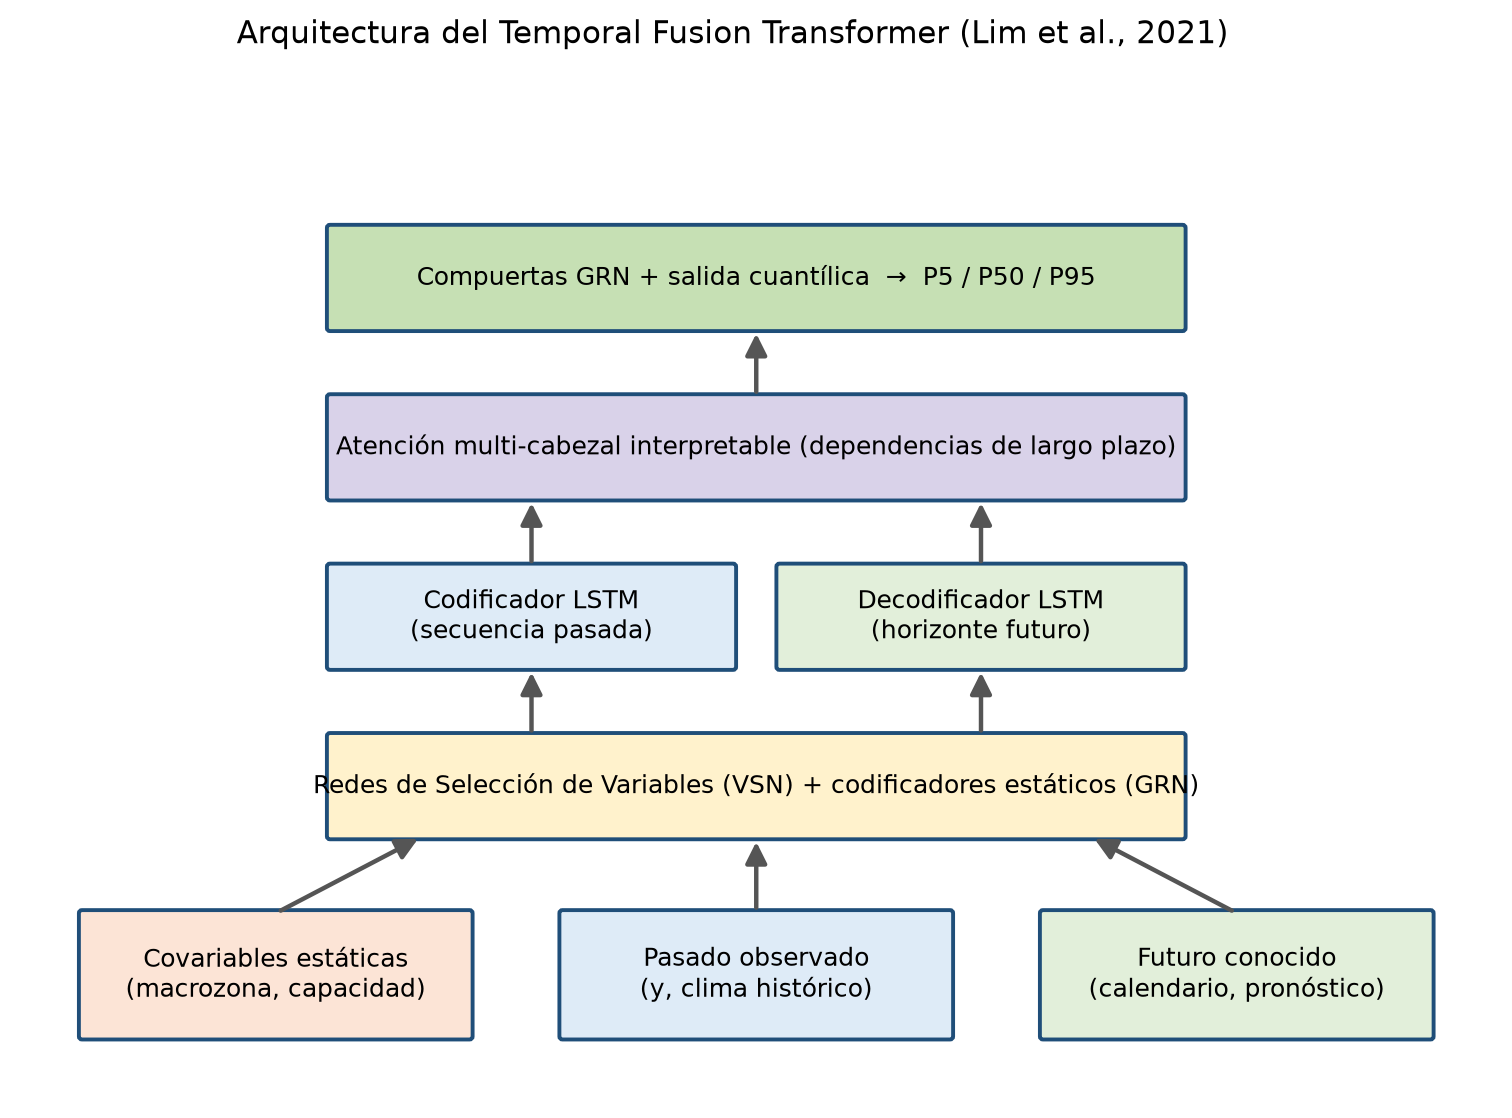
\includegraphics[width=0.82\textwidth]{figuras/fig_tft_arch.png}
  \caption{\label{fig:arquitectura_tft} Arquitectura del Temporal Fusion Transformer, destacando sus compuertas Gated Residual Networks (GRN) y su bloque de atención multipunto.}
\end{figure}

\subsection{Del Paradigma Local al Global: Aprendizaje Multi-Sitio}
Todas las técnicas anteriores pueden desplegarse bajo dos paradigmas de entrenamiento fundamentalmente distintos. En el enfoque \textbf{local} (\textit{one-site}), se ajusta un modelo independiente por cada serie temporal, utilizando exclusivamente su propio historial; es el supuesto operativo tradicional de los modelos estadísticos. En el enfoque \textbf{global} (\textit{multi-site}), un único modelo se entrena de forma simultánea sobre un conjunto de múltiples series, aprendiendo patrones compartidos y regularidades transversales al conjunto \cite{MonteroManso2021}. La evidencia empírica reciente indica que, en conjuntos de series relacionadas y especialmente bajo condiciones de intermitencia o cortes de telemetría, el paradigma global aporta un efecto estabilizador y una mejor generalización que su contraparte local \cite{Damato2026}.

Este paradigma global se materializa a través del \textbf{aprendizaje por transferencia} (\textit{Transfer Learning}), técnica en la que el conocimiento extraído de la resolución de una tarea con abundancia de datos se reutiliza para resolver un problema análogo en un dominio con escasez de datos \cite{PanYang2010}. Aplicado al pronóstico solar, esta concepción adopta la forma de \textbf{aprendizaje multi-sitio} (\textit{Cross-Site Learning}): un modelo de Deep Learning se entrena con la ingesta simultánea de datos de un clúster de plantas fotovoltaicas geográficamente distribuidas y, al correlacionar sus atributos estáticos con las variables dinámicas globales, abstrae el comportamiento atmosférico fundamental subyacente. El modelo resultante puede así emitir pronósticos para una planta nueva reduciendo o eliminando la exigencia de un historial local sustancial.

\begin{figure}[hbt!]
  \centering
  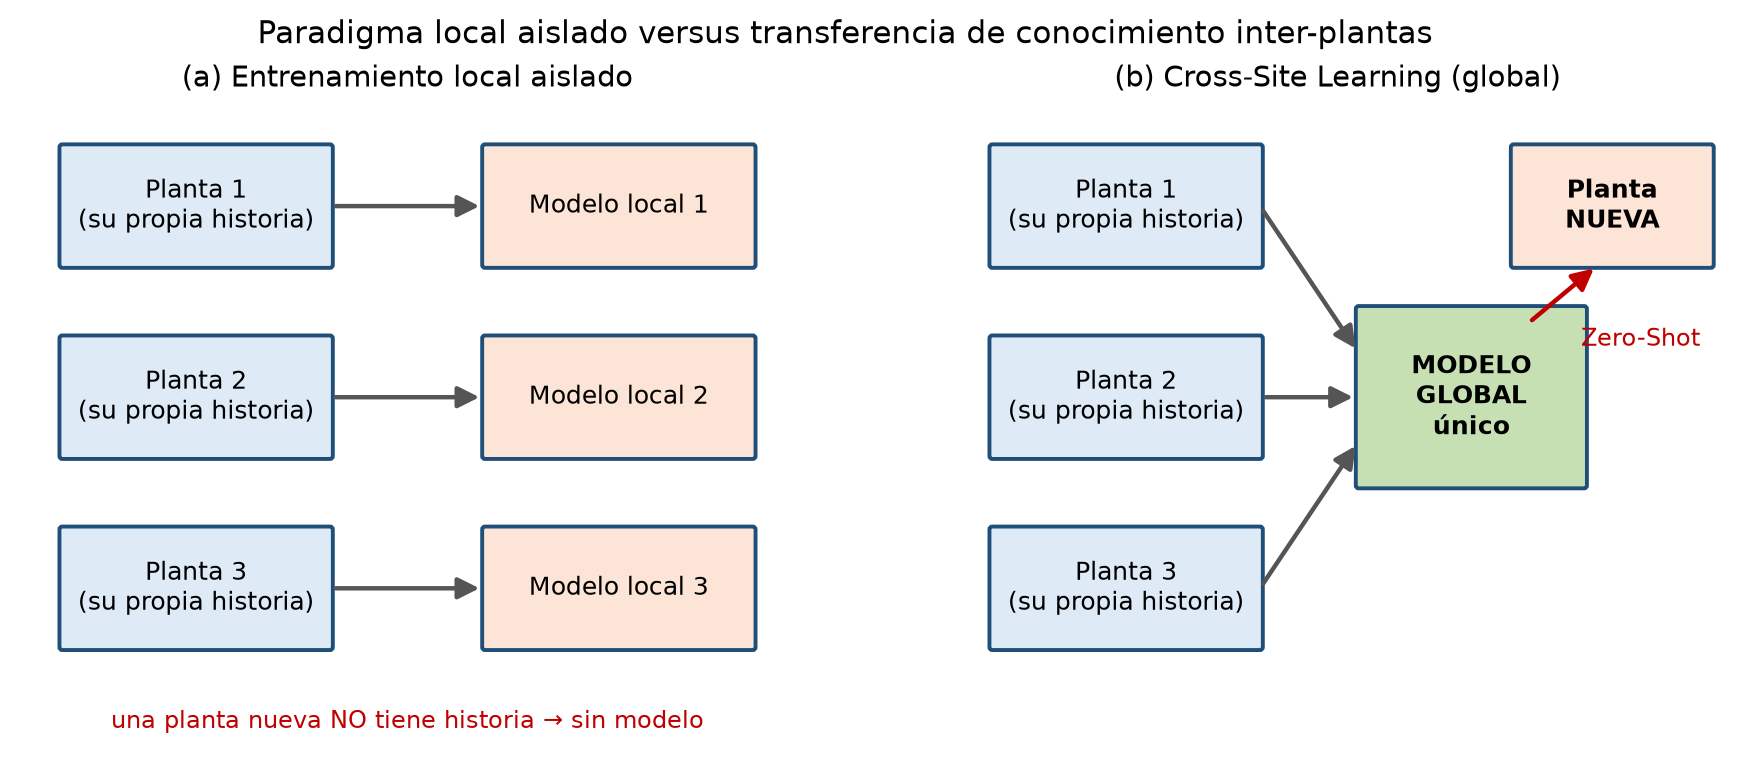
\includegraphics[width=\textwidth]{figuras/fig_cross_site.png}
  \caption{\label{fig:cross_site} Flujo conceptual de transferencia de conocimiento global inter-plantas versus el entrenamiento local y aislado.}
\end{figure}

\subsection{El Problema del Arranque en Frío (Cold-Start)}
El concepto de \textit{Cold-Start} (arranque en frío), originado en los sistemas de recomendación y trasladado al ámbito de las energías renovables, se refiere a la incapacidad de un algoritmo predictivo para generar estimaciones confiables debido a la ausencia parcial o total de datos históricos locales en una instalación recién puesta en marcha \needcite{problema de Cold-Start en pronóstico de energía / sistemas de recomendación}. Dado que los modelos locales —estadísticos, de \textit{Machine Learning} y de \textit{Deep Learning}— requieren extensos registros para modelar la estacionalidad climática anual y evitar el sobreajuste, la fase inicial de operación de un nuevo parque solar se caracteriza por una alta degradación predictiva que impacta la estabilidad de la red de transmisión. El aprendizaje multi-sitio se postula, precisamente, como la vía para transferir el conocimiento climático generalizado de la flota operativa hacia estas instalaciones sin historia.

\subsection{Conclusión acerca de las Herramientas Seleccionadas}
A partir de la revisión precedente queda sustentado el arreglo metodológico del proyecto. Como arquitecturas globales de \textit{Deep Learning} para ejecutar el paradigma \textit{Cross-Site} se seleccionan el \textbf{Temporal Fusion Transformer} (TFT), la arquitectura atencional \textbf{Informer} y la red jerárquica \textbf{N-HiTS}, complementadas por una \textbf{LSTM} global. Como líneas base del paradigma local tradicional se emplean \textbf{XGBoost} y las mismas arquitecturas profundas entrenadas de forma estrictamente aislada por planta. Este contraste —modelos globales frente a modelos locales, sobre un protocolo de evaluación idéntico— provee el marco analítico riguroso necesario para cuantificar empíricamente en qué medida el aprendizaje multi-sitio mitiga el problema del \textit{Cold-Start} bajo escasez informativa extrema.


\chapter*{Capítulo III\\Estado del Arte / Benchmarking}
\addcontentsline{toc}{chapter}{\chaptername{} III}
  
\section{Estado del Arte / Benchmarking}
Este capítulo revisa la literatura científica reciente centrada específicamente en la \textbf{aplicación} de técnicas de aprendizaje al pronóstico de generación fotovoltaica. A diferencia del marco teórico —que expuso la genealogía de los métodos—, aquí el interés recae en cómo esos métodos se han instrumentado sobre datos solares reales, qué desempeño empírico han reportado y qué limitaciones persisten. La revisión avanza de lo general a lo específico: parte de los enfoques de \textit{Machine Learning} y aprendizaje profundo aplicados al pronóstico solar, transita hacia las arquitecturas atencionales, y converge en la frontera que motiva esta investigación: la transferencia de conocimiento entre plantas bajo escasez de datos.

\subsection{Enfoques de Machine Learning y Aprendizaje Profundo en el Pronóstico Fotovoltaico}
La investigación aplicada inicial del pronóstico fotovoltaico se apoyó predominantemente en algoritmos ajustados con el historial climático de una sola ubicación. En una evaluación comparativa sobre un conjunto de datos solar real, Arslan et al. (2025) contrastaron algoritmos clásicos de \textit{Machine Learning} frente a modelos de aprendizaje profundo basados en Transformers, documentando la superioridad de estos últimos para capturar la dinámica no lineal de la irradiancia, aunque a costa de un mayor requerimiento computacional y de datos \cite{Arslan2025}. En la misma línea, los estudios centrados en algoritmos de potenciación del gradiente han consolidado a XGBoost como una línea base robusta y explicable para el pronóstico energético, destacando su eficiencia y su capacidad para jerarquizar la importancia de las variables meteorológicas, si bien evidencian su fragilidad ante regímenes de datos no observados en entrenamiento \cite{rodriguez2023energy}. Estos trabajos establecen el punto de partida empírico: los modelos locales son eficaces sobre bancos de datos extensos, pero su desempeño se degrada precisamente en las condiciones de escasez que caracterizan la puesta en marcha de una planta.

\subsection{Arquitecturas Atencionales Aplicadas a la Energía Solar}
La adopción de arquitecturas Transformer en el dominio solar ha producido resultados consistentemente favorables. López Santos et al. (2022) aplicaron el \textit{Temporal Fusion Transformer} al pronóstico fotovoltaico a un día vista (\textit{day-ahead}), aprovechando su capacidad para fusionar covariables estáticas y dinámicas y para emitir predicciones por cuantiles, y reportaron mejoras significativas frente a las líneas base recurrentes \cite{LopezSantos2022}. El-Saieed (2025) propuso un Transformer adaptativo para el pronóstico de largo plazo de temperatura y radiación en el contexto de la generación fotovoltaica, mostrando la idoneidad del mecanismo de atención para modelar las dependencias meteorológicas de largo alcance que gobiernan la producción \cite{ElSaieed2025}. Ampliando el espectro de fuentes de datos, Li et al. (2024) abordaron el \textit{nowcasting} solar mediante un Transformer que ingiere imágenes de satélite geoestacionario, evidenciando que la atención puede explotar información espacial exógena para anticipar la variabilidad inducida por la nubosidad \cite{Li2024}. En conjunto, esta línea confirma que las arquitecturas atencionales constituyen el estado del arte metodológico en el pronóstico fotovoltaico aplicado, pero la mayoría de estos trabajos opera todavía bajo el supuesto de disponer de historial local suficiente para el entrenamiento.

\subsection{Transferencia de Conocimiento y Escasez de Datos en Sistemas Fotovoltaicos}
La frontera de la disciplina, y el núcleo de esta investigación, es la aplicación de la transferencia de conocimiento para resolver la escasez de datos. Bak et al. (2025) testearon empíricamente esquemas de \textit{Transfer Learning} para el pronóstico de potencia fotovoltaica \textbf{entre regiones}, agregando datos de gran escala de múltiples plantas operativas para pre-entrenar un modelo base; sus resultados demuestran una atenuación de los márgenes de error durante las primeras semanas de operación en sitios geográficos nuevos, aunque el esquema aún requiere una fase de ajuste fino (\textit{fine-tuning}) una vez disponibles los primeros registros locales \cite{Bak2025}. Llevando esta idea a su expresión más extrema, Mishra et al. (2025) exploraron el pronóstico de irradiancia solar de corto plazo mediante modelos fundacionales en un régimen de \textbf{transferencia zero-shot}, es decir, sin ajuste alguno sobre la planta objetivo, anticipando el potencial de los modelos pre-entrenados a gran escala para operar desde el primer instante \cite{Mishra2025}. Estos trabajos validan la dirección del aprendizaje multi-sitio, pero dejan abierta la pregunta de cuánto de esa ganancia se sostiene bajo un protocolo de evaluación estrictamente ciego a la planta objetivo y contrastado de forma justa contra líneas base locales maduras.

\subsection{Síntesis Comparativa y Brecha Identificada}
La Tabla \ref{tab:benchmarking} sintetiza los estudios revisados según su enfoque, aporte principal y limitación metodológica.

\begin{table}[htbp]
  \centering
  \resizebox{\textwidth}{!}{
  \begin{tabular}{|m{3.2cm}|m{3.3cm}|m{4.5cm}|m{4.5cm}|}
    \hline
    \textbf{Estudio} & \textbf{Enfoque} & \textbf{Aporte principal} & \textbf{Limitación metodológica} \\
    \hline
    Arslan et al. (2025) & ML vs.\ Transformer (local) & Comparación empírica sobre datos solares reales; superioridad de la atención. & Entrenamiento local; no aborda el arranque en frío. \\
    \hline
    Zhu et al.\ (XGBoost) & Machine Learning local & Línea base robusta y explicable para pronóstico energético. & Degradación severa fuera del rango histórico observado. \\
    \hline
    López Santos et al. (2022) & TFT para FV (\textit{day-ahead}) & Fusión de covariables estáticas/dinámicas y pronóstico por cuantiles. & Requiere historial local del sitio evaluado. \\
    \hline
    El-Saieed (2025) & Transformer adaptativo FV & Modelado de dependencias meteorológicas de largo plazo. & Enfocado en variables meteorológicas, no en transferencia inter-sitio. \\
    \hline
    Li et al. (2024) & Transformer + satélite & Explotación de información espacial exógena (nubosidad). & Dependencia de infraestructura de datos satelitales. \\
    \hline
    Bak et al. (2025) & Transfer Learning inter-regional & Atenuación del error en las primeras semanas en sitios nuevos. & Exige \textit{fine-tuning} con datos locales iniciales. \\
    \hline
    Mishra et al. (2025) & Zero-shot / modelo fundacional & Pronóstico de irradiancia sin ajuste sobre el sitio objetivo. & Foco en irradiancia; sin \textit{benchmarking} contra locales maduros. \\
    \hline
  \end{tabular}
  }
  \caption{\label{tab:benchmarking} Síntesis comparativa de los estudios de pronóstico fotovoltaico aplicado revisados.}
\end{table}

De la revisión emerge una brecha clara. Si bien la literatura valida tanto la eficacia de las arquitecturas atencionales sobre datos solares como la promesa del aprendizaje por transferencia para mitigar la escasez de datos, los trabajos existentes rara vez combinan tres condiciones simultáneamente: \textbf{(i)} una evaluación estrictamente ciega a la planta objetivo (\textit{zero-shot} real, sin ajuste ni contexto local), \textbf{(ii)} un contraste directo y justo contra líneas base locales maduras bajo un protocolo idéntico, y \textbf{(iii)} una caracterización de la incertidumbre mediante intervalos probabilísticos y un análisis de sensibilidad estacional. La mayoría, además, opera sobre pocas plantas o requiere fases de ajuste fino que difuminan la condición de arranque en frío puro.

Para abordar esta brecha, el presente proyecto de título implementa y evalúa un marco predictivo \textit{Cross-Site} soportado sobre el \textit{Temporal Fusion Transformer}, el \textit{Informer} y N-HiTS, bajo un protocolo de retención de una planta (\textit{Leave-One-Plant-Out}) que garantiza la integridad \textit{zero-shot}. La evaluación se estructura como un \textit{benchmarking} cerrado que contrasta estas arquitecturas globales contra líneas base estrictamente locales (XGBoost y las mismas redes profundas entrenadas de forma aislada), reporta métricas puntuales y probabilísticas, y estratifica los resultados por estación del año sobre un conjunto de \textbf{94 plantas fotovoltaicas} del Sistema Eléctrico Nacional chileno. Esta configuración permite dictaminar cuantitativamente en qué medida el conocimiento climático generalizado de la flota operativa mitiga los sesgos predictivos durante el arranque en frío de nuevos parques solares.


\chapter*{Capítulo IV\\Metodología y Propuesta de Solución}
\addcontentsline{toc}{chapter}{\chaptername{} IV}

\section{Metodología y Propuesta de Solución}

\subsection{Propuesta de Solución}
La propuesta de solución consiste en el diseño e implementación de un modelo predictivo global basado en una arquitectura Transformer, el cual es pre-entrenado mediante un enfoque \textit{Cross-Site Learning} sobre un conglomerado de plantas solares consolidadas. El propósito central es transferir este conocimiento climático hacia instalaciones nuevas que sufren de escasez de datos e intermitencias operativas (\textit{Cold-Start}), logrando proyecciones estables desde sus primeros días de conexión a la red.

Con base en los requerimientos técnicos de integridad informativa, el alcance empírico abarca instalaciones solares consolidadas y agrupadas estratégicamente por Macrozona. En lugar de limitar la muestra a un número fijo de plantas en una única región, el enfoque \textit{Cross-Site} capitaliza la diversidad geográfica y climática disponible, empleando algoritmos de imputación robustos para aquellos vacíos operativos manejables. Esta configuración garantiza que el modelo asimile una correlación termodinámica auténtica y representativa, permitiendo transferir el aprendizaje a nuevas instalaciones independientemente de su ubicación, siempre que compartan el perfil macrozonal.
Desde la perspectiva algorítmica, el proyecto adopta la arquitectura \textit{Temporal Fusion Transformer} (TFT) debido a su capacidad innata para procesar de forma asimétrica datos multimodales: asimilando variables dinámicas meteorológicas temporales en conjunto con características estáticas geográficas. Para dictaminar la efectividad de esta red frente a la problemática de arranque en frío, se contrastará su rendimiento de extrapolación (\textit{Zero-Shot}) frente a otras arquitecturas globales de \textit{Deep Learning} (\textit{Informer} y \textit{N-HiTS}, junto a un \textit{XGBoost} global) y contra líneas base estrictamente locales (\textit{XGBoost}, \textit{LSTM} y \textit{N-HiTS} entrenadas de forma aislada por planta), conformando un total de ocho configuraciones evaluadas bajo un protocolo idéntico.

\begin{figure}[htbp]
  \centering
  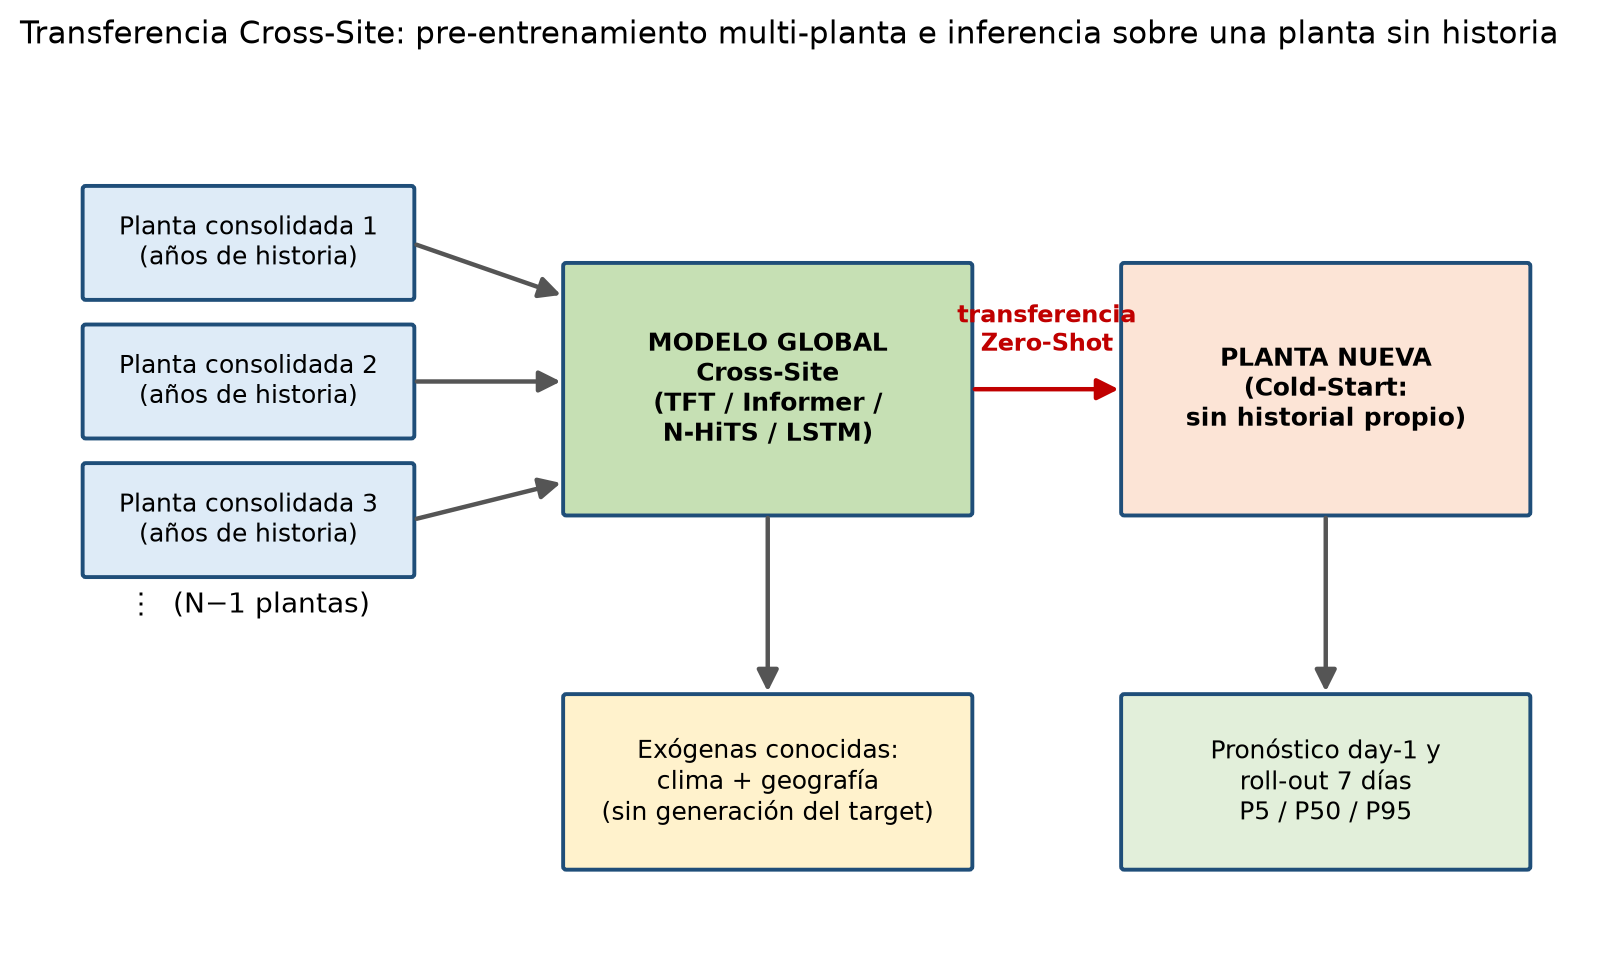
\includegraphics[width=\textwidth]{figuras/fig_solucion.png}
  \caption{\label{fig:diagrama_solucion} Representación esquemática de la propuesta de solución predictiva.}
\end{figure}

\subsection{\label{p:adaptacion}Adaptación Metodológica (Pipeline de Trabajo)}
Para sistematizar la ejecución del proyecto y asegurar la replicabilidad de los experimentos, la investigación se apoya en un \textit{pipeline} de \textit{Machine Learning Operations} (MLOps) segmentado en cuatro fases metodológicas secuenciales implementadas en lenguaje Python.

\subsubsection{Fase 0: Extracción, Transformación y Carga (ETL)}
La fase fundacional del orquestador aborda el acondicionamiento integral de los datos estructurando el proceso en un modelo de capas secuenciales \textit{Medallion} (Landing, Bronze, Silver y Gold). Para mitigar los cortes de sensores y evitar el \textit{Data Leakage}, se definieron reglas estrictas:
\begin{enumerate}
    \item \textbf{Variables Exógenas y Agrupación:} La imputación de variables meteorológicas se realiza escalonadamente (interpolación lineal y \textit{ffill}/\textit{bfill} por grupos temporales), y se incorpora una variable indicadora booleana (\textit{dummy}) para señalar registros imputados. Además, se aplican características cíclicas (\textit{seno/coseno}) para capturar estacionalidad y se impone un forzamiento a cero en la irradiancia global durante períodos nocturnos garantizados.
    \item \textbf{Manejo Estricto del Target (Intocable):} A diferencia de las variables exógenas, la variable objetivo (generación de energía) no es sometida a ningún tipo de imputación ni se rellena con ceros lógicos. Si un registro horario está ausente, permanece como NaN en el vector final. Los modelos administran estas intermitencias mediante la reindexación de la grilla horaria, y las métricas penalizan exclusivamente sobre observaciones reales y existentes. Esta decisión asegura que el \textit{Performance Ratio} no se distorsione sintéticamente.
\end{enumerate}

\begin{figure}[htbp]
  \centering
  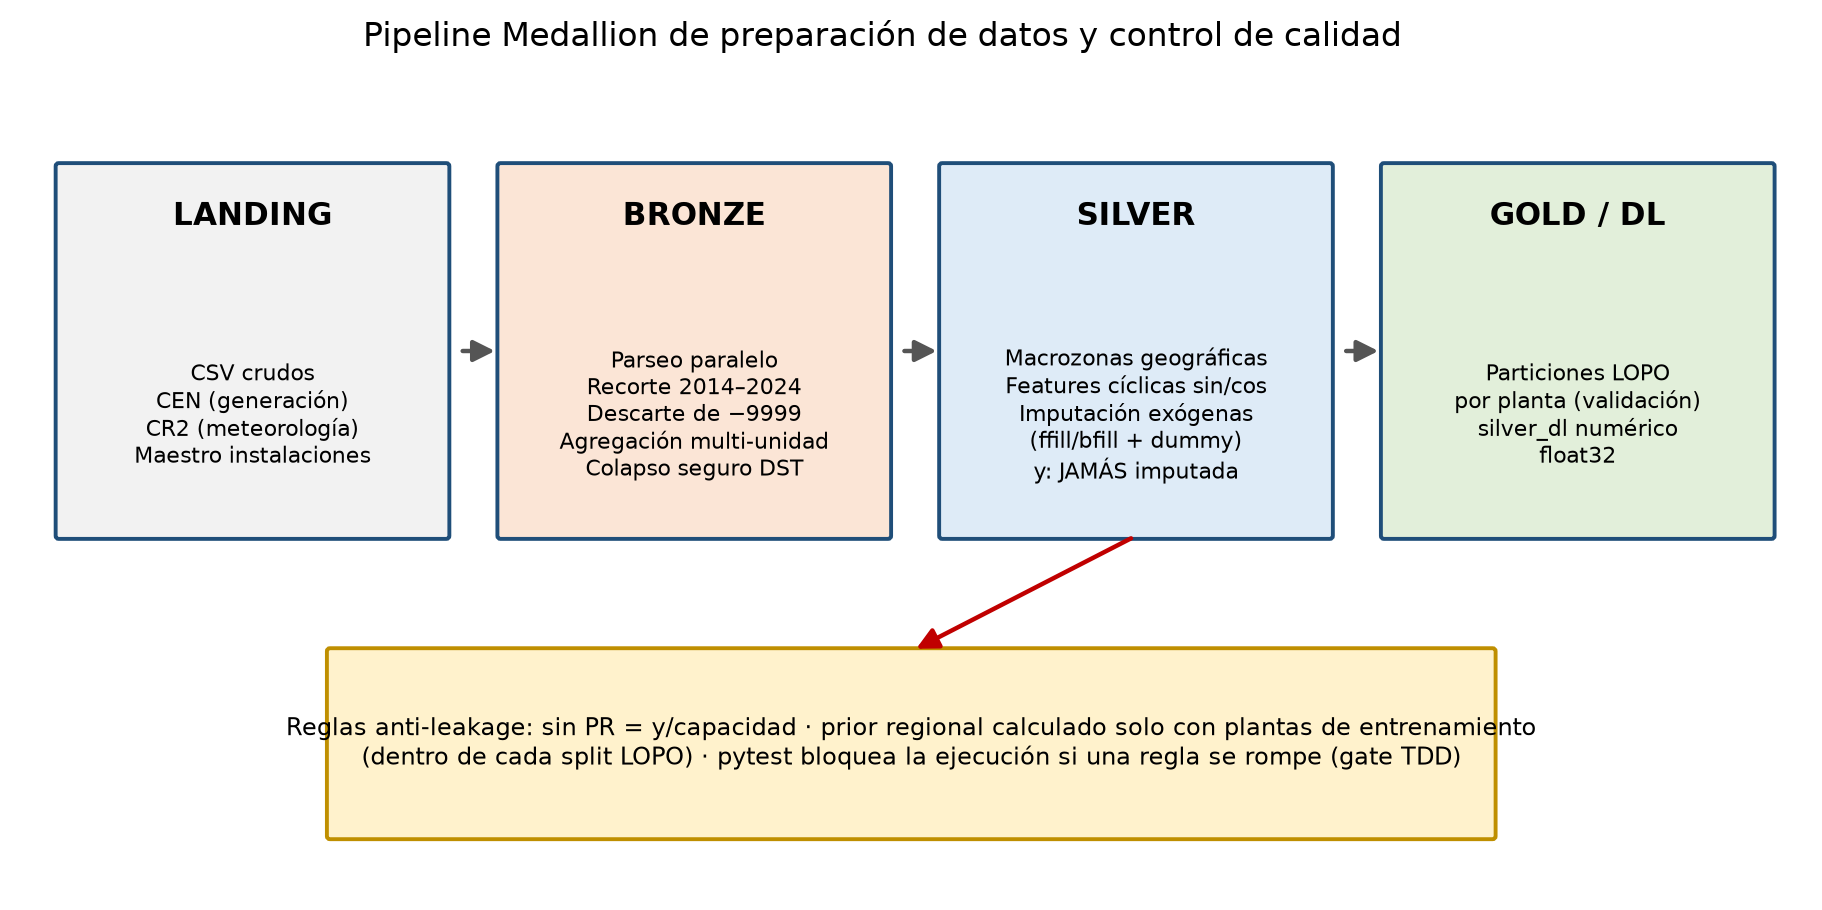
\includegraphics[width=\textwidth]{figuras/fig_etl_flow.png}
  \caption{\label{fig:etl_flow} Algoritmia del proceso de preparación de datos y control de calidad.}
\end{figure}

\subsubsection{Fase 1: Sintonización de Hiperparámetros (Tuning)}
Para garantizar una comparativa justa (\textit{Benchmarking}) entre las redes profundas globales y los algoritmos tradicionales locales, es imperativo descubrir la configuración óptima de la topología de las redes. En esta etapa, el orquestador emplea heurísticas de búsqueda y validación cruzada para sintonizar los hiperparámetros críticos (tasa de aprendizaje, profundidad del codificador, número de cabezales de atención en el TFT y tamaño de la ventana temporal) maximizando el rendimiento predictivo inicial sobre el corpus histórico general antes de someter a los modelos al estrés del arranque en frío.

\subsubsection{Fase 2: Simulación Cold-Start (Estrategia LOPO)}
El núcleo de la experimentación reside en la aplicación de la metodología de retención espacial \textit{Leave-One-Plant-Out} (LOPO). En lugar de dividir el set de datos cronológicamente, el orquestador aísla dinámicamente y oculta por completo el historial operativo de una de las plantas (capa \textit{Gold} de validación). 
El modelo \textit{Cross-Site} es entrenado exclusivamente con los años de experiencia del resto de la flota operativa. Para emular el arranque en frío (\textit{Cold-Start}) de la planta seleccionada, el contexto histórico (\textit{seed}) previo al horizonte de pronóstico se inicializa de forma 100\% sintética ($y = \text{capacidad} \times \text{PR regional} \times \text{perfil solar}$), garantizando así que no exista \textit{Data Leakage}. Dicho coeficiente de \textit{Performance Ratio (PR) regional} se calcula como un agrupamiento histórico estratificado por Macrozona y Estación del Año, computado empleando única y estrictamente el conjunto de entrenamiento. Una vez consolidados los pesos sinápticos, la red es forzada a inferir el comportamiento energético futuro de la planta oculta utilizando únicamente sus coordenadas estáticas y el clima entrante. Este procedimiento se repite iterativamente rotando la instalación objetivo. Asimismo, la orquestación de esta fase admite la ejecución bajo distintas escalas (\textit{Toy}, \textit{Half} y \textit{Total}) que modulan la fracción de la muestra analizada, agilizando el \textit{benchmarking}.

\begin{figure}[htbp]
  \centering
  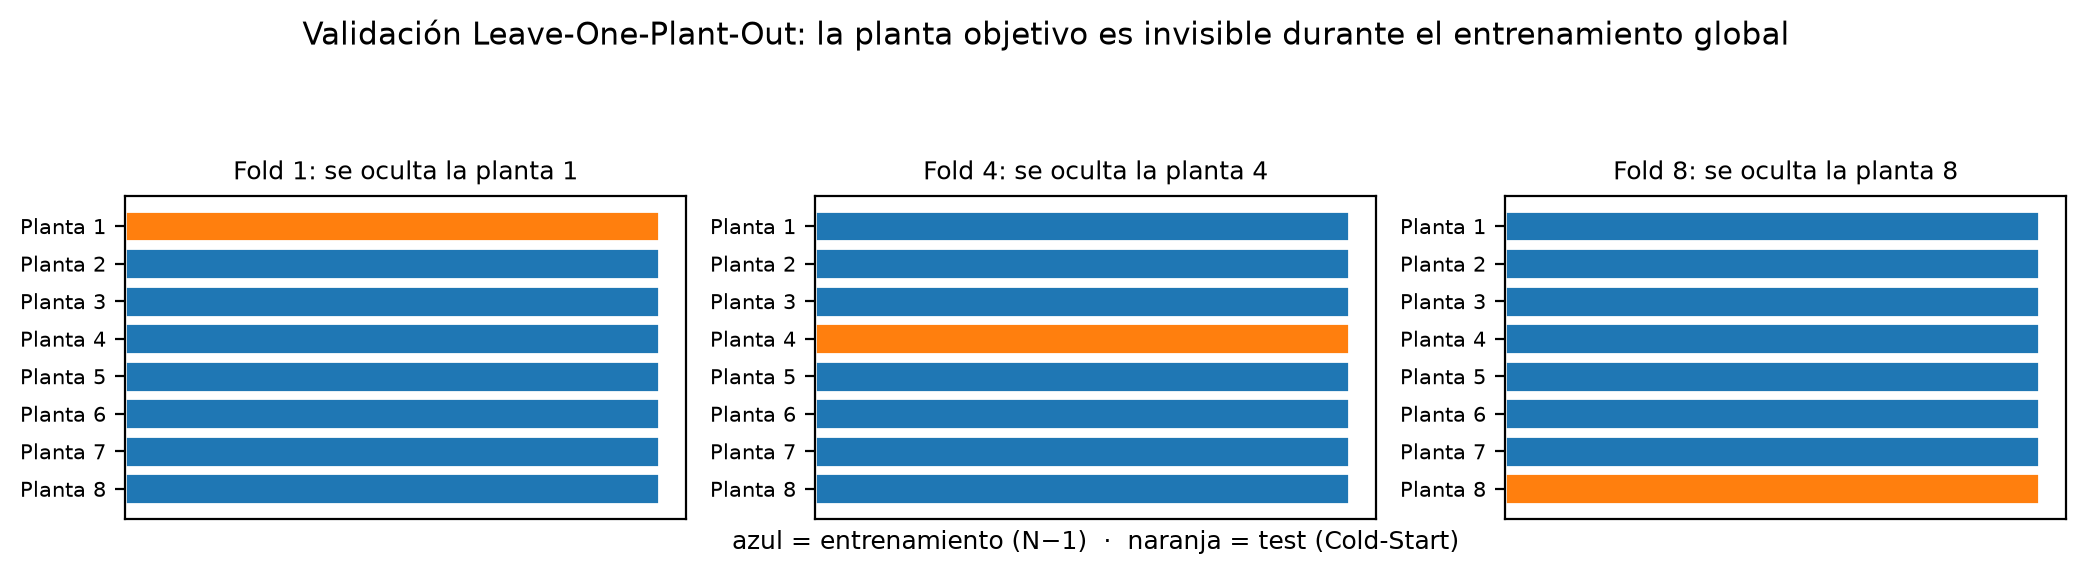
\includegraphics[width=\textwidth]{figuras/fig_lopo.png}
  \caption{\label{fig:lopo_strategy} Visualización iterativa del aislamiento espacial para simulación de arranque en frío.}
\end{figure}

\subsubsection{Fase 3: Extracción de Resultados y Métricas de Rendimiento}
La fase final consolida los vectores predictivos generados por cada una de las arquitecturas sometidas a prueba —modelos globales \textit{Cross-Site} (TFT, Informer, N-HiTS, LSTM y XGBoost Global) y líneas base estrictamente locales entrenadas con la historia propia de cada planta (XGBoost, LSTM y N-HiTS locales)— contrastándolos unificadamente contra la producción energética empírica de los parques solares aplicando 2 estrategias de testeo diferenciadas según la ventana temporal proyectada (\textit{day1} para predicción a 24 horas y \textit{rollout7d} para proyección expandida iterativa a una semana).
Adicionalmente, los resultados y desvíos son evaluados de manera estratificada según la \textbf{Estación del Año}, lo que permite medir el impacto de la variabilidad meteorológica cíclica en las redes. El proyecto computa métricas clásicas de pronóstico, entre las cuales destacan:
\begin{itemize}
    \item \textbf{Error Absoluto Medio (MAE):} Para cuantificar la magnitud promedio lineal del error en la escala energética real (MW).
    \item \textbf{Error Cuadrático Medio (RMSE):} Para penalizar cuadráticamente las desviaciones más grandes generadas por los sesgos del modelo durante picos de inyección, dado que eleva al cuadrado cada error antes de promediarlo.
    \item \textbf{Error Porcentual Absoluto Medio Simétrico (sMAPE):} Empleado como estándar de industria para dimensionar la falla en términos relativos porcentuales, independientemente de la capacidad instalada de la planta.
    \item \textbf{Pronóstico Probabilístico:} los modelos emiten intervalos de predicción del 90\,\% (cuantiles P5/P50/P95) para reportar la incertidumbre esperada. Su calidad se evalúa mediante dos indicadores distintos: la \textbf{cobertura empírica}, definida como la frecuencia con que la observación real cae dentro del intervalo (idealmente cercana al 90\,\% nominal), y la \textbf{pérdida pinball} (\textit{pinball loss}), una función de costo cuantílica que penaliza de forma asimétrica los errores por encima y por debajo de cada cuantil. Las predicciones finales se ajustan para cumplir leyes físicas (mínimo de cero general y cero estricto de noche).
\end{itemize}
La consolidación de estas métricas se tabulará y graficará para facilitar el análisis comparativo financiero y operativo entre el modelo Transformer global y las líneas base locales.

\begin{figure}[htbp]
  \centering
  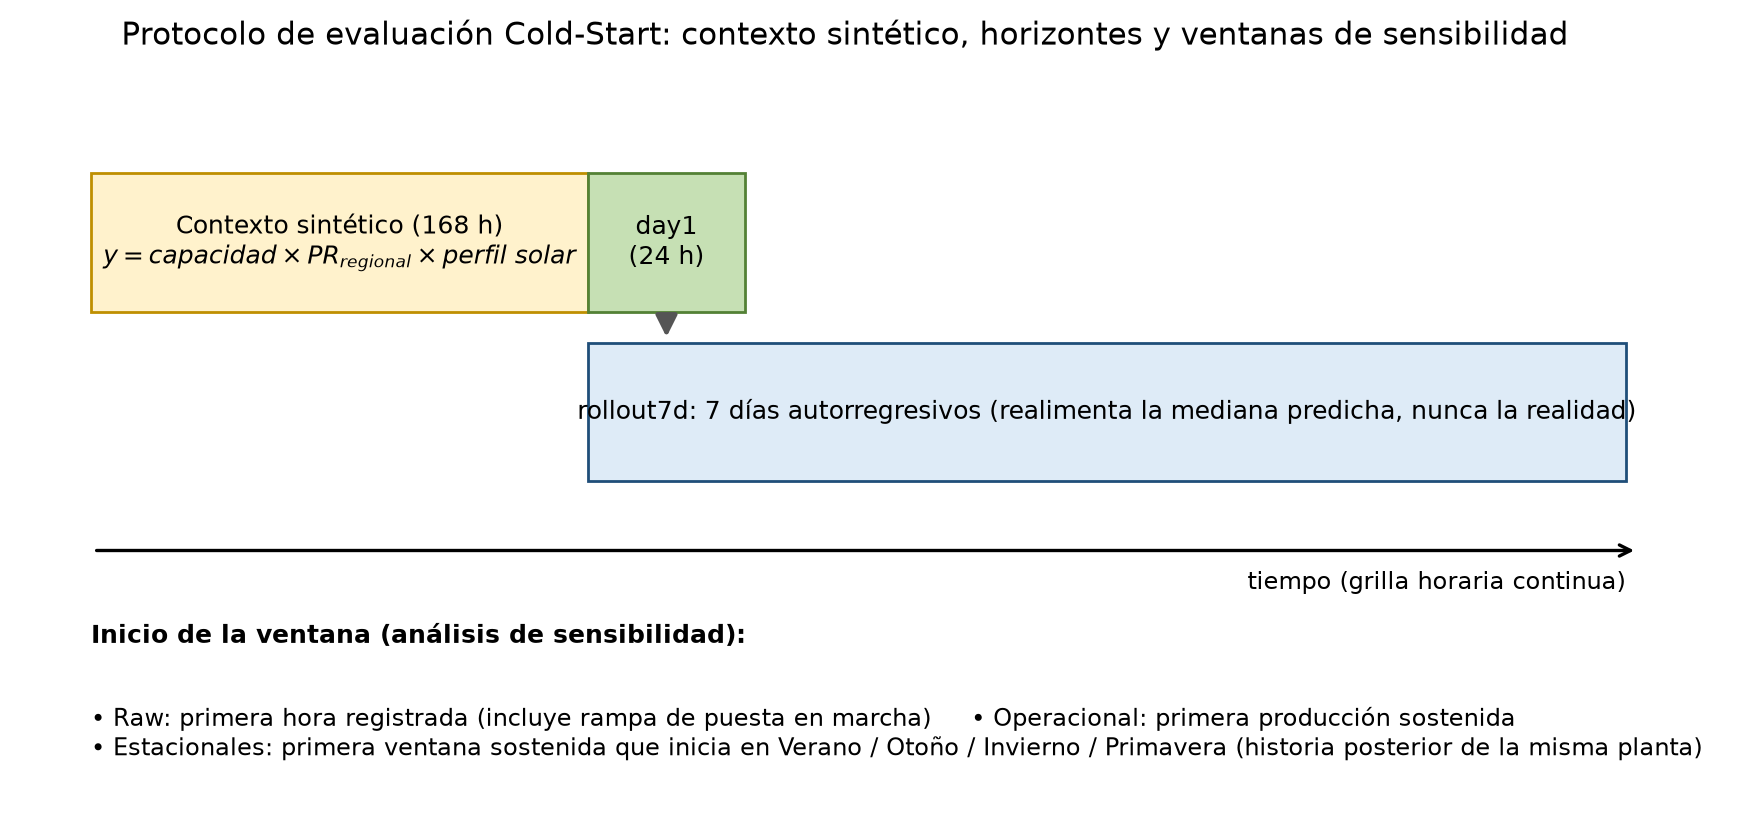
\includegraphics[width=\textwidth]{figuras/fig_eval_protocolo.png}
  \caption{\label{fig:metrics_visual} Protocolo de evaluación Cold-Start: contexto sintético, horizontes de pronóstico y ventanas del análisis de sensibilidad sobre las cuales se computan las métricas comparativas.}
\end{figure}

El cronograma temporal que ordena la ejecución de estas cuatro fases corresponde a la carta Gantt de seis semanas presentada en la Figura \ref{fig:gantt_planificacion} del Capítulo I, cuyas actividades se encuentran categorizadas según el objetivo específico al que tributan.

\subsection{Arquitectura de Componentes y Stack Tecnológico}
Más allá del flujo lógico de datos descrito en las fases anteriores, la solución se materializa como un sistema de software modular gobernado por un \textbf{orquestador único} (\texttt{src/orchestrator.py}), que constituye el único punto de entrada de producción y coordina la ejecución secuencial de las capas del \textit{pipeline}. La Figura \ref{fig:arquitectura} presenta el diagrama de componentes, la estructura de módulos y el \textit{stack} tecnológico sobre el que se implementa cada etapa.

La primera capa, \textbf{ETL} (\texttt{src/etl/}), materializa el flujo Medallion: los módulos \texttt{landing\_\allowbreak to\_\allowbreak bronze} ingieren y normalizan los archivos crudos de generación y meteorología, \texttt{bronze\_\allowbreak to\_\allowbreak silver} aplica el agrupamiento por macrozona, las variables cíclicas y la imputación auditada de exógenas, y \texttt{silver\_\allowbreak to\_\allowbreak gold\_\allowbreak split} particiona los conjuntos de prueba por planta; el módulo \texttt{prepare\_\allowbreak dl\_\allowbreak dataset} deriva la versión numérica del conjunto apta para las redes profundas. La segunda capa, \textbf{ML} (\texttt{src/\allowbreak ml/\allowbreak orchestrator\_\allowbreak ml.py}), ejecuta el bucle \textit{Leave-One-Plant-Out}: para cada planta objetivo entrena y evalúa las cinco arquitecturas globales sobre las $N-1$ plantas restantes (con el ciclo \textit{tune}$\rightarrow$\textit{train}$\rightarrow$\textit{test}) y, en paralelo, las tres líneas base estrictamente locales. La tercera capa, \textbf{Reporte}, consolida las métricas y genera las figuras y tablas del presente documento. Las tres capas se apoyan en un conjunto de \textbf{utilidades compartidas} (\texttt{src/\allowbreak ml/\allowbreak utils/}) que centralizan la lógica sensible a la integridad científica —el particionado LOPO (\texttt{data\_\allowbreak loader}), la grilla horaria canónica (\texttt{grid}), la definición de ventanas (\texttt{eval\_\allowbreak window}), el \textit{prior} regional (\texttt{regional\_\allowbreak prior}) y el cómputo de métricas (\texttt{metrics})—, evitando su duplicación y garantizando un tratamiento idéntico para todos los modelos.

El orquestador incorpora, además, dos salvaguardas de ingeniería: un \textit{gate} de pruebas automatizadas (\texttt{pytest}) que se ejecuta antes de cada corrida y detiene el \textit{pipeline} ante cualquier fallo, y un control de idempotencia mediante marcadores de completitud que permite reanudar ejecuciones largas sin recomputar trabajo ya finalizado. El \textit{stack} tecnológico se compone de Python 3.12 como lenguaje base, PyArrow/Parquet para la persistencia columnar entre capas, pandas para la manipulación tabular, el ecosistema NeuralForecast de Nixtla sobre PyTorch 2.5.1 (CUDA 12.1) para las arquitecturas profundas, XGBoost para los modelos de árboles, Optuna para la optimización de hiperparámetros y matplotlib/seaborn para la visualización.

\begin{figure}[htbp]
  \centering
  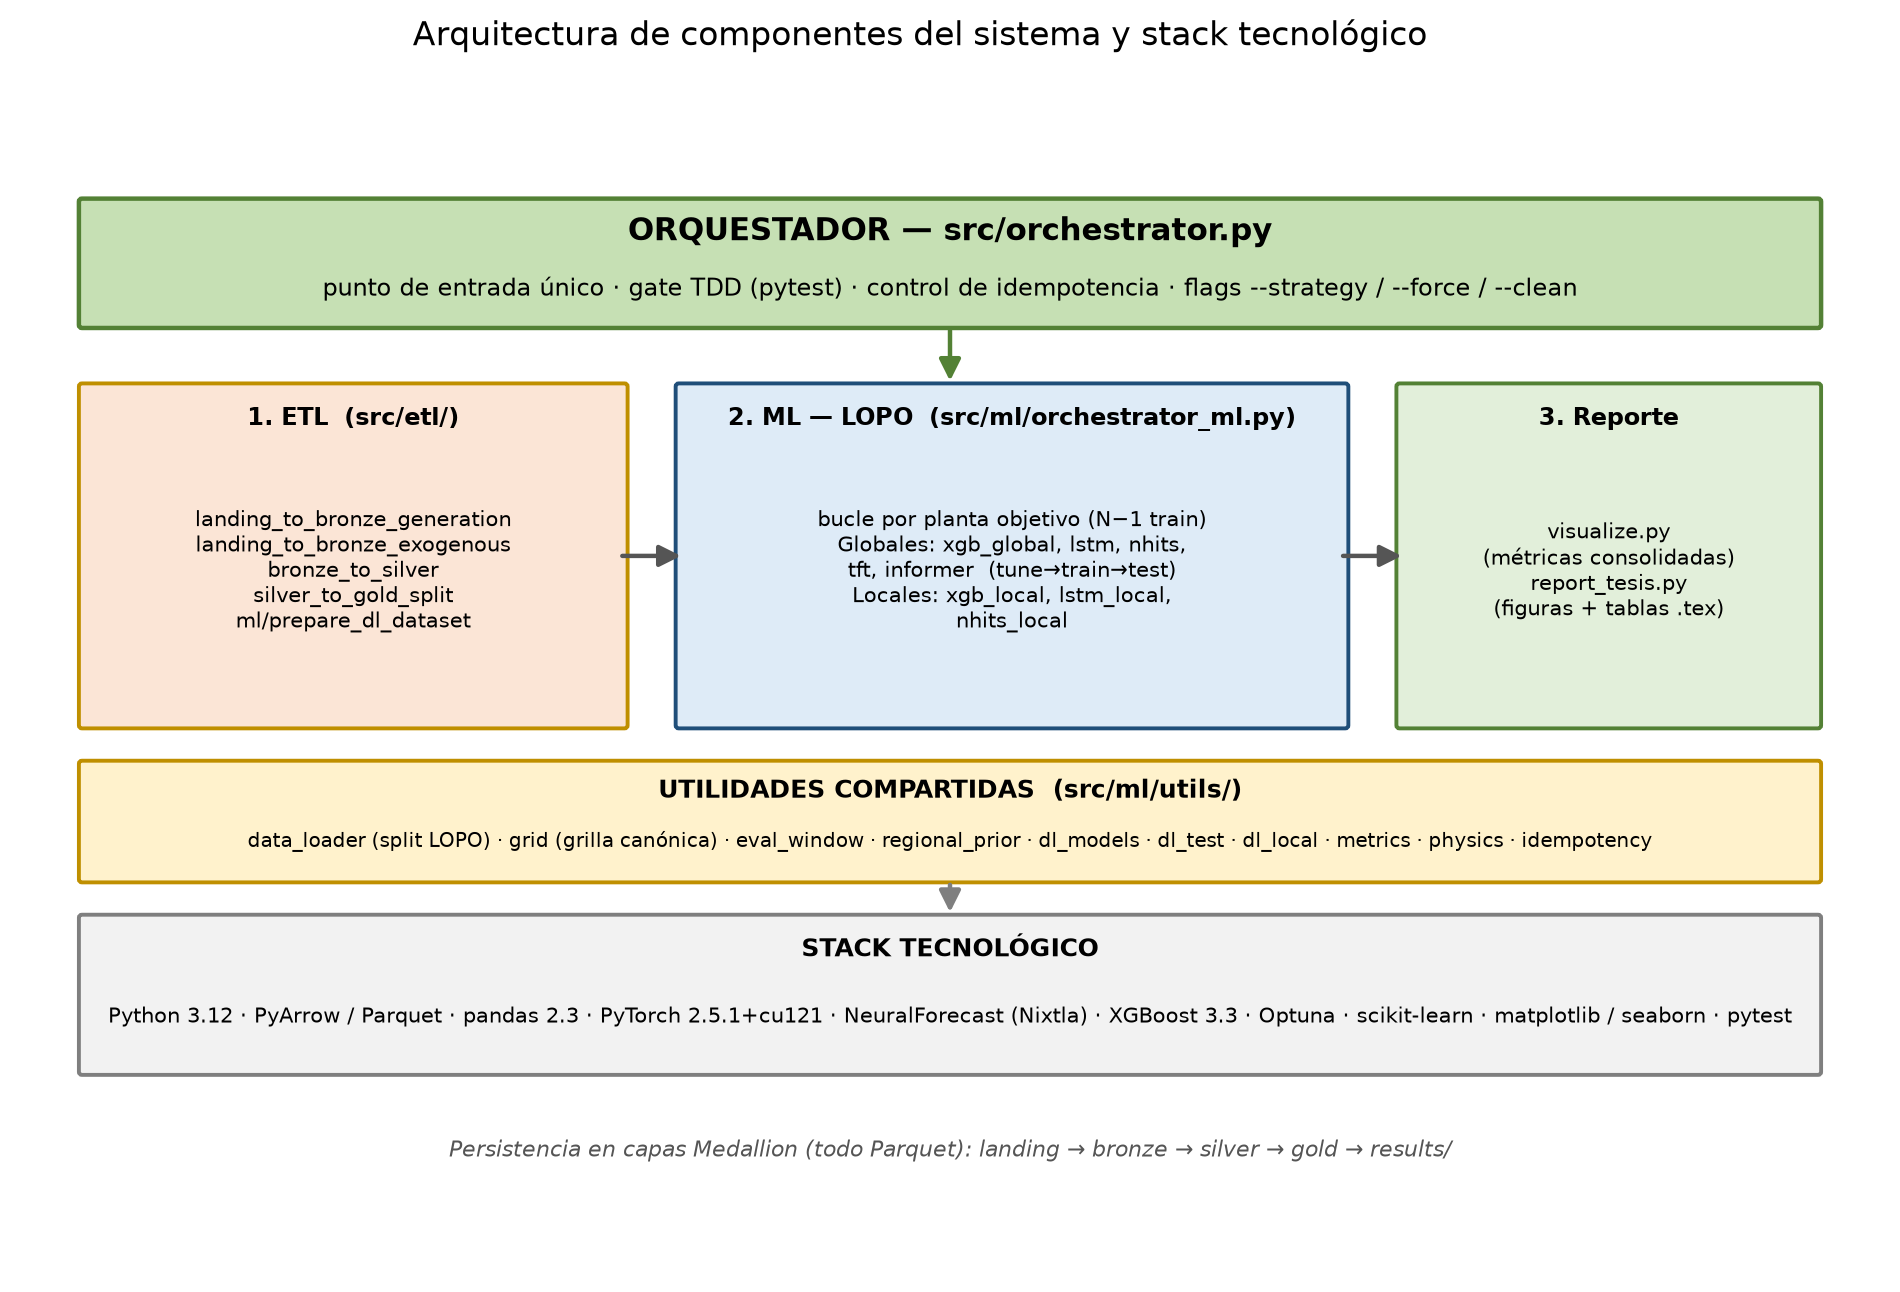
\includegraphics[width=\textwidth]{figuras/fig_arquitectura_componentes.png}
  \caption{\label{fig:arquitectura} Diagrama de componentes del sistema: orquestador único, las tres capas del \textit{pipeline} (ETL, ML--LOPO y Reporte) con sus módulos, la capa de utilidades compartidas y el \textit{stack} tecnológico que soporta cada etapa.}
\end{figure}

\FloatBarrier
\subsection{Estudio de Factibilidad}

\subsubsection{Factibilidad técnica}
La factibilidad técnica de este proyecto está garantizada por la disponibilidad de herramientas de \textit{software} de código abierto (\textit{Open Source}) y librerías especializadas en \textit{Machine Learning} y \textit{Deep Learning}. Toda la orquestación del pipeline (ETL, entrenamiento y validación) se encuentra programada en \textit{Python}, utilizando el ecosistema \textit{Nixtla} (específicamente \textit{NeuralForecast}) para la ejecución de los algoritmos atencionales de última generación (TFT y N-HiTS), así como \textit{XGBoost} para las líneas base locales. Adicionalmente, el procesamiento matricial intensivo requerido por el paradigma \textit{Cross-Site Learning} se aborda mediante el uso de aceleración por hardware computacional (GPUs), recursos que son accesibles a través de entornos de desarrollo estándar.

\subsubsection{Factibilidad operativa}
La operación del estudio es autónoma y reproducible: el pipeline completo se ejecuta desde un único punto de entrada con validación automatizada previa (gate de pruebas), control de idempotencia para reanudar corridas interrumpidas y generación automática de reportes. La extensión del análisis a nuevas plantas o períodos no requiere infraestructura ni personal adicional.

\subsubsection{Factibilidad económica}
El costo marginal del proyecto es prácticamente nulo: las fuentes de datos son públicas (Coordinador Eléctrico Nacional y red climatológica CR2), la totalidad del software empleado es de código abierto y el cómputo se resuelve en hardware de consumo (una única GPU de gama media), sin requerir financiamiento externo ni servicios de nube de pago.

\subsubsection{Factibilidad legal}
Los datos empleados provienen de repositorios públicos de organismos oficiales chilenos y no contienen datos personales ni información sujeta a confidencialidad. Las licencias de las librerías utilizadas (ecosistema Python de código abierto) son compatibles con el uso académico e investigativo del presente trabajo.

\subsubsection{Factibilidad Social}
El proyecto no genera impactos sociales adversos. Indirectamente, la mejora del pronóstico de generación en plantas recién conectadas contribuye a la estabilidad del suministro eléctrico y reduce las barreras de entrada para nuevos actores renovables de menor escala.

\subsubsection{Factibilidad Ambiental}
La investigación tributa a la descarbonización de la matriz energética al facilitar la integración temprana de nueva capacidad solar. La huella de cómputo del estudio es acotada: los entrenamientos completos se resuelven en horas sobre una única GPU, sin infraestructura de centros de datos dedicada.

\chapter*{Capítulo V\\Desarrollo de la Propuesta y Resultados}
\addcontentsline{toc}{chapter}{\chaptername{} V}
\section{Desarrollo de la Propuesta y Resultados}

Considere que en este apartado debe demostrar el desarrollo de la propuesta del capítulo anterior con los resultados obtenidos en cada fase.

\begin{itemize}
\item Debe incorporar los apartados de cada etapa declarada y evidencias más importantes del desarrollo, con los resultados obtenidos en cada uno de ellos, el resto de las evidencias de cada una de las fases, deben pasar a los Anexos.
\item \colorbox{yellow}{Borre el texto que no sea suyo} y comience a escribir en ese punto.
\end{itemize}

\subsubsection{Etapa1 del desarrollo}

\subsubsection{Etapa 2 del desarrollo}

\subsubsection{Etapa X del desarrollo}

Documentar cada una de las partes del desarrollo de su propuesta, de acuerdo con la carta gantt y los elementos comprometidos en el capítulo anterior, hasta llegar al resultado, con los elementos más importantes, el resto debe quedar en evidencia como anexo a este documento.

\chapter*{Capítulo VI\\Conclusiones y Trabajo Futuro}
\addcontentsline{toc}{chapter}{\chaptername{} VI}

\section{Conclusiones y Trabajo Futuro}

% [PENDIENTE: párrafo introductorio breve del capítulo una vez consolidados
%  los resultados de la corrida HALF/TOTAL.]

\subsubsection{Conclusiones}
% [PENDIENTE: redactar en tercera persona a partir de los resultados de la
%  Fase 3 (Capítulo V). Estructura sugerida alineada con la rúbrica
%  (relación resultados-metodología-objetivos):
%   1. Cumplimiento del Objetivo Específico 1 (arquitectura Transformer
%      adaptada al entrenamiento multi-serie con exógenas multimodales).
%   2. Cumplimiento del Objetivo Específico 2 (evaluación Cold-Start LOPO
%      global vs. baselines locales) y veredicto sobre la HIPÓTESIS del
%      Capítulo I.
%   3. Cumplimiento del Objetivo Específico 3 (integración multimodal:
%      exógenas dinámicas + estáticas geográficas).
%   4. Hallazgos metodológicos relevantes: rampas de puesta en marcha y
%      sensibilidad de la ventana de evaluación; efecto estacional
%      (dificultad invernal); integridad del target sin imputación.]

\subsubsection{Trabajos Futuros}
% [PENDIENTE: redactar fundamentado en los resultados. Candidatos ya
%  identificados durante el desarrollo:
%   - Ajuste fino (fine-tuning) del modelo global con los primeros días de
%     datos reales de la planta nueva (transfer learning en dos etapas).
%   - Incorporación de PatchTST cuando el ecosistema NeuralForecast
%     incorpore soporte de variables exógenas para dicha arquitectura.
%   - Extensión del prior regional de eficiencia con clustering climático
%     más fino que la Macrozona.
%   - Despliegue operacional (MLOps) explícitamente excluido del alcance.]


\clearpage
\phantomsection
\addcontentsline{toc}{chapter}{Bibliografía}
\fancyhead[L]{BIBLIOGRAFÍA}
\bibliographystyle{apalike}
\begingroup
\makeatletter
% Eliminar el espacio gigante del título usando comportamiento de sección
\let\chapter\section
% Forzar viñeta de punto para cada entrada
\def\@lbibitem[#1]#2{\item[\textbullet]\if@filesw
      {\let\protect\noexpand
       \immediate
       \write\@auxout{\string\bibcite{#2}{#1}}}\fi\ignorespaces}
\makeatother
\bibliography{bibliografia}
\endgroup

\chapter*{Anexos}
\addcontentsline{toc}{chapter}{Anexos}
\fancyhead[L]{ANEXOS}
\renewcommand\thesection{\Alph{section}}
\setcounter{section}{0}
\section{Repositorio del Proyecto}
El código fuente completo del proyecto (pipelines de datos, entrenamiento, evaluación LOPO y generación de reportes), junto a su suite de pruebas automatizadas, se encuentra versionado en un repositorio Git.
% [PENDIENTE: URL del repositorio o referencia al medio de entrega.]

\section{Tablas Completas de Métricas por Planta}
% [PENDIENTE: exportar desde results/<estrategia>/visuals/all_metrics_summary.csv
%  las tablas completas por planta, ventana de evaluación, estación y horizonte.]

\section{Registro de Imputación de Variables Exógenas}
% [PENDIENTE: resumen estadístico del log de imputación de la capa Silver
%  (data/silver/imputation_log.csv): proporción imputada por variable y macrozona.]

\section{Hallazgos de Calidad de Datos}
% [PENDIENTE: detalle de los hallazgos documentados en el Capítulo V, Fase 0:
%  agregación multi-unidad (PFV Jama), transiciones DST y rampas de puesta
%  en marcha por planta.]


\end{document}